\documentclass[a4paper, amsfonts, amssymb, amsmath, reprint, showkeys,
nofootinbib, twoside]{revtex4-2}
\usepackage{preamble}

\begin{document}

    \title{Étude du Chaos, Caractérisation des Attracteurs Chaotiques}

    \author{Antoine de Lagrave}
    \affiliation{
        Université de Sherbrooke, Département de physique, Sherbrooke, QC,
        Canada
    }
    \date{\today}

    \begin{abstract}
        Dans ce travail, nous étudions la caractérisation des attracteurs
        chaotiques des systèmes dynamiques. Les attracteurs chaotiques
        présentent un comportement complexe, imprévisible et non périodique,
        et constituent une caractéristique fondamentale des systèmes non
        linéaires dissipatifs. Nous utilisons diverses méthodes pour
        identifier et analyser les attracteurs chaotiques, incluant le calcul
        de(s) exposant(s) de Lyapunov. L'utilisation de méthodes numériques
        comme des algorithmes de résolution d'équations différentielles sera
        impérative et précieuse dans l'analyse numérique de tels système, de
        même que l'utilisation d'algorithme de convergence pour obtenir une
        intuition de leur comportement après un temps qui tend vers l'infini.
        Nous présentons également des exemples de ce type d'attracteurs tels
        que : l'attracteur de Lorenz, l'attracteur de Rössler, l'attracteur de
        Bouali et etc. Notre étude révèle ainsi la structure riche et complexe
        des attracteurs chaotiques et fournit des aperçus sur la dynamique
        sous-jacente des systèmes qui sont à l'origine de leur apparition.
        Dans l'ensemble, cette étude contribue à une compréhension plus
        approfondie du chaos et fournit des aperçus pour l'analyse des
        systèmes chaotiques en utilisant les attracteurs comme entité
        principale.
    \end{abstract}

    \maketitle

    \section{Introduction} \label{sec: introduction}

L'intérêt scientifique envers les systèmes chaotiques remonte au 19\up{ème}
siècle alors que Henri Poincaré étudiait le comportement des solutions du
problème à trois corps \cite{poin_carre}. Bien qu'il n'était pas évident que
ce système était de nature chaotique, la forte sensibilité aux conditions
initiales et la non périodicité des solutions étaient toutefois très présentes.
Birkhoff, Kolmogorov et Lorenz sont également d'éminents mathématiciens et
physiciens qui ont plus tard contribué considérablement dans le domaine de la
théorie du chaos respectivement grâce à la théorie ergodique, l'étude des
turbulences/algorithmes et l'étude de la météorologie. C'est d'ailleurs Edward
Lorenz qui en 1963, arrive avec l'idée \textit{l'effet papillon} selon lequel
de légères variations peuvent avoir des conséquences monstrueuses
\cite{butterfly}. Ce n'est cependant qu'au 20\up{ème} siècle que ce sujet
d'étude à connu ses plus grandes victoires et avancées. La raison principale
de cette ascension est la croissance fulgurante de l'ère numérique. L'étude de
tels systèmes est en effet particulièrement coûteuse en ce qui concerne la
partie mathématique puisqu'elle demande une grande quantité d'itérations et
c'est pourquoi les ordinateurs y sont d'une aide précieuse.

L'étude des systèmes dynamiques dissipatifs requiert régulièrement
l'intervention d'outils mathématiques et topologiques complexes pour être en
mesure d'isoler une tendance ou un comportement physique. On entend ici par
\textit{systèmes dynamiques dissipatifs} des systèmes thermodynamiques qui
agissent hors équilibre et dans lesquels les échanges d'énergie et de matière
avec l'environnement sont permis. Ces systèmes sont donc ouverts au sens
thermodynamique et sont généralement à l'origine de l'apparition d'attracteurs.
Plus précisément, les systèmes dynamiques dont la sensibilité aux conditions
initiales est élevée sont aussi appelés systèmes chaotiques. Ceux-ci sont à la
fois déterministes et imprévisibles et c'est ce mélange particulier de
simplicité et de hasard qui constitue le \textit{chaos} Il sera ici question
d'étudier les différentes propriétés et limites de certains attracteurs
fondamentaux qui émergent naturellement des systèmes dynamiques dissipatifs
tels que l'attracteur de Lorenz, Rössler et Bouali. On déterminera leur
sensibilité aux conditions initiales via l'exposant de Lyapunov. Nous
pourrons ainsi faire un lien entre ces attracteurs et de réels systèmes
physiques dans lesquels ont retrouve ces objets topologiques naturellement.


    \section{Théorie} \label{sec: theory}
    Les attracteurs sont des structures fondamentales en théorie du chaos qui
    jouent un rôle clé dans la compréhension du comportement chaotique des
    systèmes. Dans cette section, nous allons explorer en détail le concept
    d'attracteur en théorie du chaos, en examinant les propriétés mathématiques
    qui les caractérisent.

\subsection{Attracteurs} \label{subsec: attractors}
    Pour un système dynamique dissipatif donné, l'attracteur est définit par
    un sous-ensemble d'états dans l'espace des phases vers lesquels la
    solution au système converge si les conditions initiales de ladite solution
    sont comprises dans le bassin d'attraction de l'attracteur. Ici, le
    \textit{bassin d'attraction} représente une zone de l'espace des phases
    dont les conditions initiales mènent à des trajectoires qui convergent vers
    un attracteur. Mathématiquement, on dit que le bassin d'attraction $W$
    d'un attracteur $A$ est
    \begin{align}
        W(A) = \{r\in R\;\;|\;\lim_{t\to\infty} f(r, t)\in A\},
    \end{align}

    où ici $r$ représente un ensemble de condition initiales appartenant à
    l'espace des phases $R$ et $f(r, t)$ la trajectoire de la solution.
    Autrement-dit, l'attracteur est un sous-ensemble de solutions qui permet
    d'identifier et de prédire une tendance globale dans la trajectoire d'une
    solution donnée d'un système chaotique, et ce, malgré sa nature
    imprévisible. \\

    L'attracteur de Lorenz que l'on nommera ici $L$ est l'un des exemples les
    plus célèbres d'un attracteur chaotique dans la théorie des systèmes
    dynamiques \cite{lorenz}. Cet attracteur est le fruit d'un système
    dynamique non linéaire à trois dimensions qui décrit le comportement d'un
    fluide en mouvement. Mathématiquement, l'attracteur de Lorenz est défini
    par un ensemble d'équations différentielles ordinaires, qui décrivent
    l'évolution de trois variables dynamiques $(x, y, z)$ en fonction du temps
    et des paramètres $\sigma, \rho$ et $\beta$ qui régissent le comportement
    du système
    \begin{align}
        L = \left\{
        \begin{array}{c}
           \Dot{x} = \sigma(y - x) \\
           \Dot{y} = x(\rho - z) - y \\
           \Dot{z} = xy - \beta z,
        \end{array}
        \right.
        \label{eq : lorenz}
    \end{align}

    où les paramètres $\sigma, \rho$ et $\beta$ sont respectivement le nombre
    de Prandtl, le nombre de Rayleigh et un coefficient géométrique quelconque.
    Un second attracteur initialement proposé par Otto Rössler en 1976 est
    l'attracteur de Rössler \cite{rossler}. Celui-ci possède une forme
    particulière et n'a qu'une seule de ses trois équations qui possède un
    terme non linéaire
    \begin{align}
        R = \left\{
        \begin{array}{c}
           \Dot{x} = -y - z \\
           \Dot{y} = x + ay \\
           \Dot{z} = b + z(x - c),
        \end{array}
        \right.
        \label{eq : rossler}
    \end{align}

    avec $a, b$ et $c$ des paramètres numériques qui régissent le comportement
    du système. Le dernier attracteur que nous allons étudier est celui
    introduit par Bouali en 2013, qui est non seulement par définition très
    sensible aux conditions initiales, mais également à la source du phénomène
    unique de chevauchement d'attracteurs \cite{bouali}. Les équations
    différentielles non-linéaires qui décrivent cet attracteur sont
        \begin{align}
        B = \left\{
        \begin{array}{c}
           \Dot{x} = \alpha x(1 - y) - \beta z \\
           \Dot{y} = -\gamma y(1 - x^2) \\
           \Dot{z} = \mu x,
        \end{array}
        \right.
        \label{eq : bouali}
    \end{align}

    où les paramètres $\alpha, \beta, \gamma$ et $\mu$ sont une fois de plus
    des coefficients numériques responsables du comportement de l'attracteur.

\subsection{Exposants de Lyapunov} \label{subsec: lyapunov}
    Nous avons définit que les systèmes dynamiques dissipatifs sensibles au
    changement infinitésimal des conditions initiales sont chaotiques et donc
    que deux trajectoires peuvent se voir diverger rapidement. Soit deux
    positions initiales de l'espace des phases $\bm{x}(t)$ et $\bm{x}(t) +
    \bm{\delta}_0$ tels que montrés sur la figure \ref{fig: theo_lyapunov}
    \begin{figure}[h!]
        \centering
        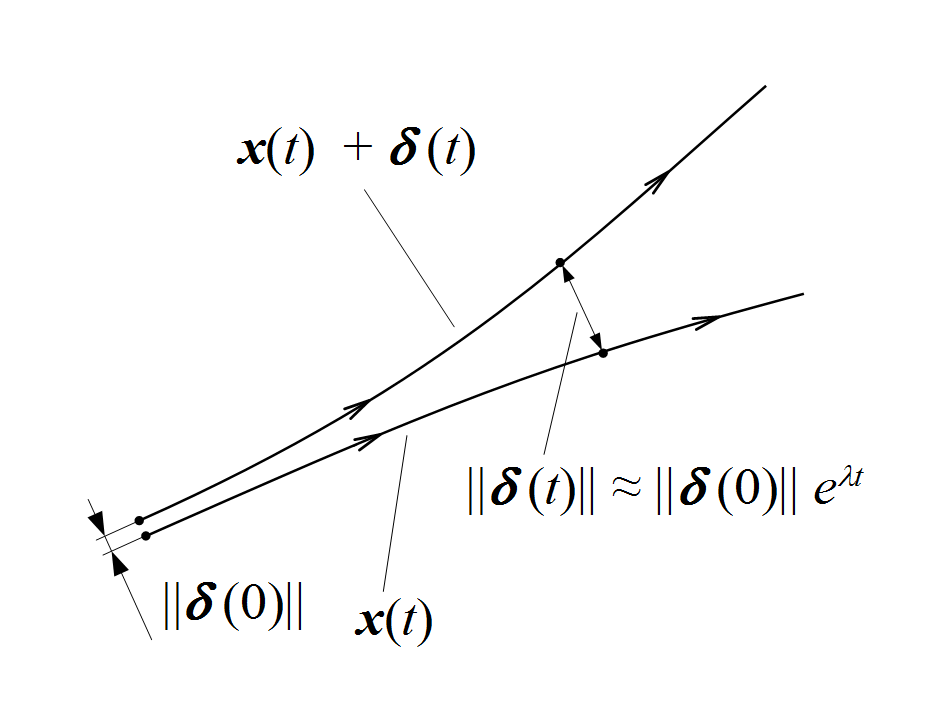
\includegraphics[scale=0.3]{figs/Orbital_instability_(Lyapunov_exponent).png}
        \caption{Schéma qui exprime l'évolution de la distance entre deux
        trajectoires $|\bm{\delta}(t)|$ initialement espacées d'un déplacement
    infinitésimal $|\bm{\delta_0}|$ en fonction du temps \cite{LEs_wiki}.}
        \label{fig: theo_lyapunov}
    \end{figure}

    on considère qu'au temps $t=0$ ces trajectoires ont été éloignées du
    vecteur déplacement $\bm{\delta}_0$ tel que sa norme $|\bm{\delta}_0|$ soit
    infinitésimale. Dans le contexte de systèmes chaotique, on trouve qu'après
    un temps d'évolution $t$, la norme du déplacement entre les trajectoires
    est donné par
    \begin{align}
        |\bm{\delta}(t)| \simeq |\bm{\delta}_0|e^{\lambda t},
        \label{eq : lyapunov_delta}
    \end{align}

    où l'on appelle la quantité $\lambda$ \textit{l'exposant de Lyapunov}. On
    accède à cette quantité avec quelques manipulation
    \begin{align}
        \lambda \simeq
        \frac{1}{t}\ln\qty[\frac{|\bm{\delta}(t)|}{|\bm{\delta}_0|}],
    \end{align}

    où pour un système avec pas temporels discrets tels que l'itération
    $x_{n + 1} = f(x_n)$, se traduit par
    \begin{align}
        \lambda(x_0) = \lim_{n\to\infty}\frac{1}{n}\sum_{i = 0}^{n - 1}\ln(f'(x_i)),
    \end{align}

    avec $x_0$ le point qui correspond à la condition initiale. On voit ici
    que pour des solutions calculées à l'aide d'algorithmes, il est possible
    de remplacer la limite itérative infinie par un algorithme de convergence
    judicieusement choisi tel que \textit{l'algorithme epsilon}. Il est
    cependant important de noter que jusqu'ici, nous n'avons introduit qu'un
    seul exposant $\lambda$ (le plus élevé conventionnellement), mais un
    système de dimension $N$ possède naturellement $N$ exposants de Lyapunov.
    On appelle ces valeurs le \textit{spectre de Lyapunov} d'un système. Ce
    spectre possède plusieurs propriétés intéressantes pour l'analyse des
    systèmes dynamiques \cite{LEs}: \\
    \begin{itemize}
        \item[$\diamond$] Les composantes du spectres sont indépendantes du
            métrique utilisé pour leur calcul ainsi que du choix des variables.
            Cela permet de conclure sur l'objectivité et la pertinence du
            spectre de Lyapunov. \\
        \item[$\diamond$] Si l'exposant le plus élevé du spectre est positif
            témoigne généralement d'instabilités exponentiellement importantes
            et consitue une définition de ce que l'on pourrait appeler chaos. \\
        \item[$\diamond$] La somme du spectre de Lyapunov permet de mesurer
            le taux contraction des volumes de l'espace des phases. Pour des
            systèmes dissipatifs, une somme $\sum_i\lambda_i < 0$ signifie que
            les volumes décroissent exponentiellement à 0 alors qu'une somme
            nulle implique la conservation des volumes de l'espace des phases.
    \end{itemize}


    \section{Théorie}

\section{Méthodes numériques}

\subsection{Équations différentielles}

\subsection{Calculs matriciels \& Convergence}

\section{Résultats}

\subsection{Trajectoires}

\subsection{Spectre de Lyapunov}

\begin{frame}
    \begin{center}
    \vspace{0.5cm}
    \boxed{
        Théorie - Équations différentielles
        }
    \end{center}
\end{frame}

\begin{frame}
    \frametitle{Théorie - Équations différentielles}
    \framesubtitle{Attracteur de Lorenz}
    Système d'équations différentielles pour l'attracteur de Lorenz \footcite{lorenz}:
    \begin{align}
            L =
            \begin{Bmatrix*}[l]
                \Dot{x} = \sigma(y - x) \\
                \Dot{y} = x(\rho - z) - y \\
                \Dot{z} = xy - \beta z
            \end{Bmatrix*},
    \end{align}
    où $\sigma, \rho$ et $\beta$ sont respectivement le nombre de Prandtl, de Rayleigh et un coefficient géométrique.
\end{frame}

\begin{frame}
    \frametitle{Théorie - Équations différentielles}
    \framesubtitle{Attracteur de Rössler}
    Système d'équations différentielles pour l'attracteur de Rössler \footcite{rossler}:
    \begin{align}
            R =
            \begin{Bmatrix*}[l]
                \Dot{x} = -y - z \\
                \Dot{y} = x + ay \\
                \Dot{z} = b + z(x - c)
            \end{Bmatrix*},
    \end{align}
    où $a, b$ et $c$ sont des coefficients géométriques quelconques.
\end{frame}

\begin{frame}
    \frametitle{Théorie - Équations différentielles}
    \framesubtitle{Attracteur de Bouali}
    Système d'équations différentielles pour l'attracteur de Bouali \footcite{bouali}:
    \begin{align}
            B =
            \begin{Bmatrix*}[l]
                \Dot{x} &= \alpha x(1 - y) - \beta z \\
                \Dot{y} &= -\gamma y(1 - x^2) \\
                \Dot{z} &= \mu x
            \end{Bmatrix*},
    \end{align}
    où $\alpha, \beta, \gamma$ et $\mu$ sont des coefficients géométriques quelconques. \vspace{0.5cm}
    \begin{noteblock}{Note}
        Le système d'équation qui modélise l'attracteur de Bouali est de degré 3 contrairement aux autres de degré 2.
    \end{noteblock}
\end{frame}

\begin{frame}
    \begin{center}
    \vspace{0.5cm}
    \boxed{
        Méthodes numériques - Équations différentielles
    }
    \end{center}
\end{frame}

\begin{frame}
    \frametitle{Méthodes numériques - Équations différentielles}
    Les méthodes de résolutions numériques utilisées sont
    \vspace{0.5cm}
    \begin{itemize}
        \setlength\itemsep{1em}
        \item[$\diamond$] Runge-Kutta d'ordre 4
        \item[$\diamond$] Librairie Python scipy (\textit{scipy.optimize.solve\_ivp()})
    \end{itemize}
    \vspace{1cm}\pause
    L'algorithme est divisé en 3 étapes: \pause
    $$
        \underbrace{\text{grille temporelle \& } \bm{r}_0}_1 \pause \to \underbrace{\text{méthode numérique}}_2 \pause \to \underbrace{\text{affichage solution}}_3
    $$
\end{frame}

\begin{frame}
    \begin{center}
    \vspace{0.5cm}
    \boxed{
        Résultats - Trajectoires
        }
    \end{center}
\end{frame}

\begin{frame}
    \frametitle{Résultats - Trajectoires}
    \framesubtitle{Attracteur de Lorenz}
    \begin{columns}
        \column{0.55\linewidth}
        \centering
        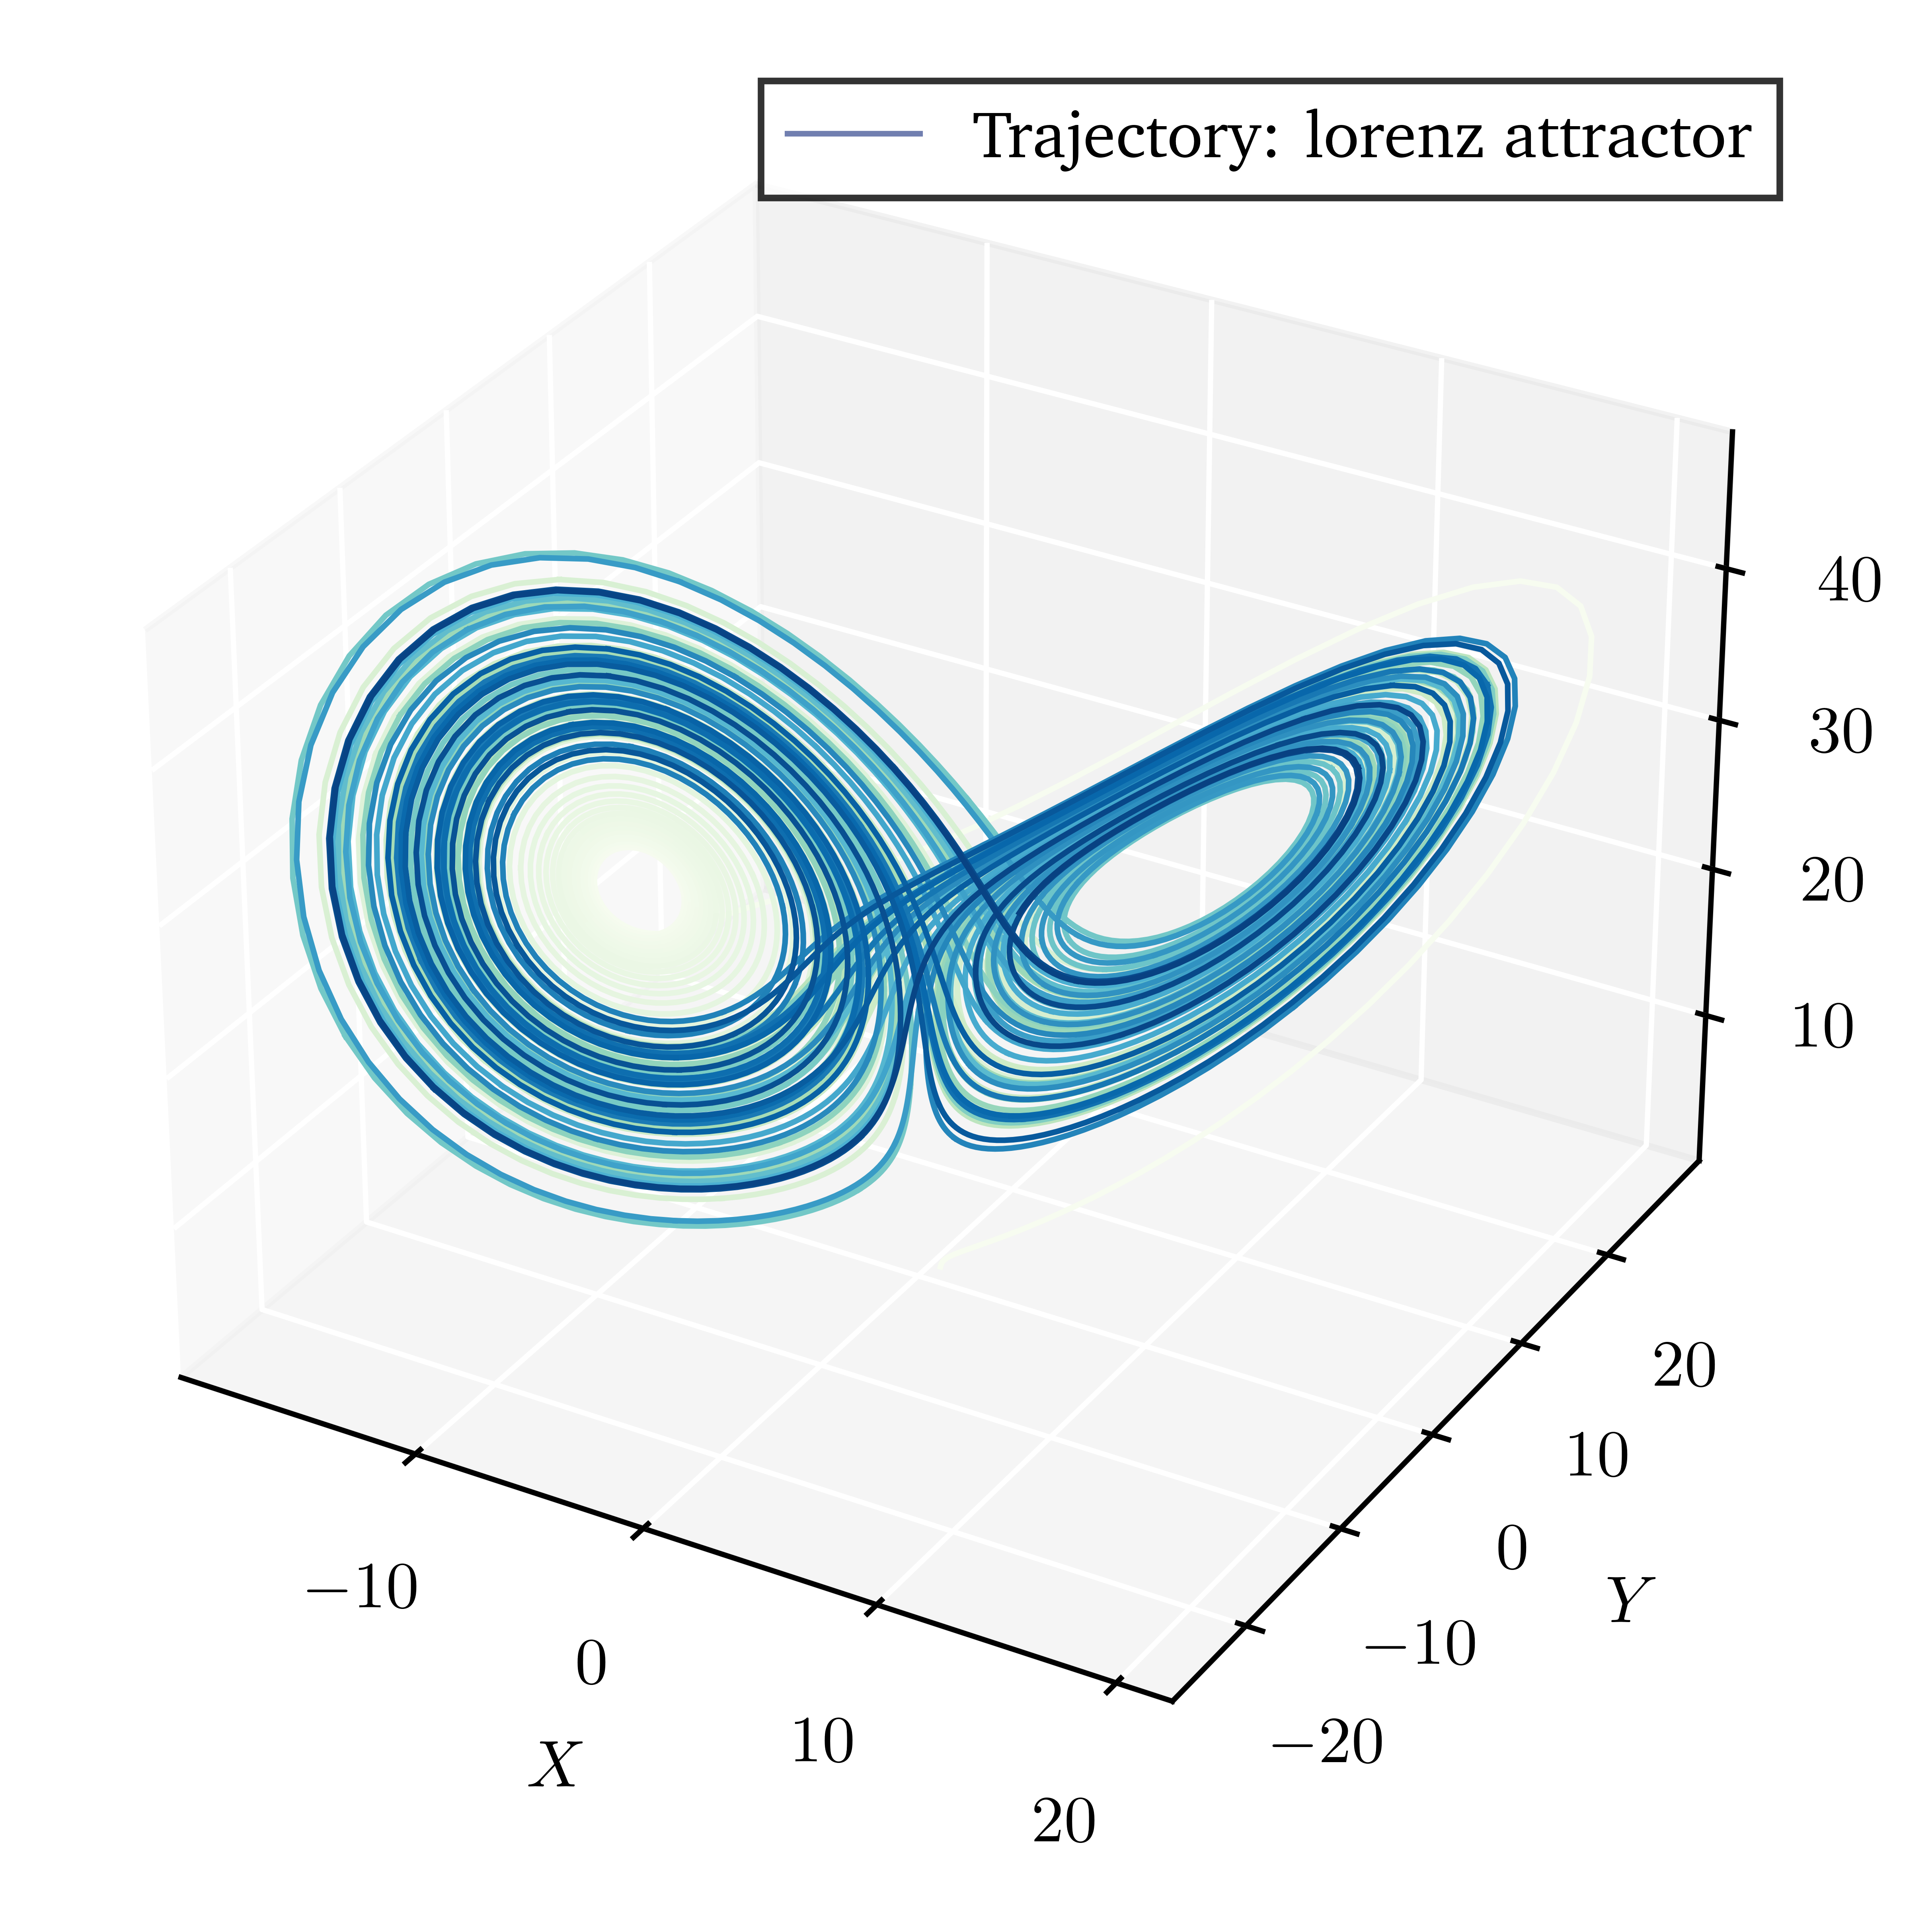
\includegraphics[scale=0.6]{figures/trajectories/traj_lorenz.png}
        \column{0.45\linewidth}
        \begin{itemize}
            \setlength\itemsep{1em}
            \item[$\diamond$] Conditions initiales $\bm{r} = (1, 0, -1)$ \\
            \item[$\diamond$] Temps de $100$ secondes
            \item[$\diamond$] Pas de $h = 0.01$
        \end{itemize}
    \end{columns}
\end{frame}

\begin{frame}
    \frametitle{Résultats - Trajectoires}
    \framesubtitle{Attracteur de Lorenz}
    \begin{columns}
        \column{0.5\linewidth}
        \centering
        \includegraphics[scale=0.55]{figures/trajectories/unicity_lorenz.png}
        \column{0.4\linewidth}
        Vérification qualitative du théorème d'unicité des solutions aux équations différentielles.
    \end{columns}
\end{frame}

\begin{frame}
    \frametitle{Résultats - Trajectoires}
    \framesubtitle{Attracteur de Rössler}
    \begin{columns}
        \column{0.55\linewidth}
        \centering
        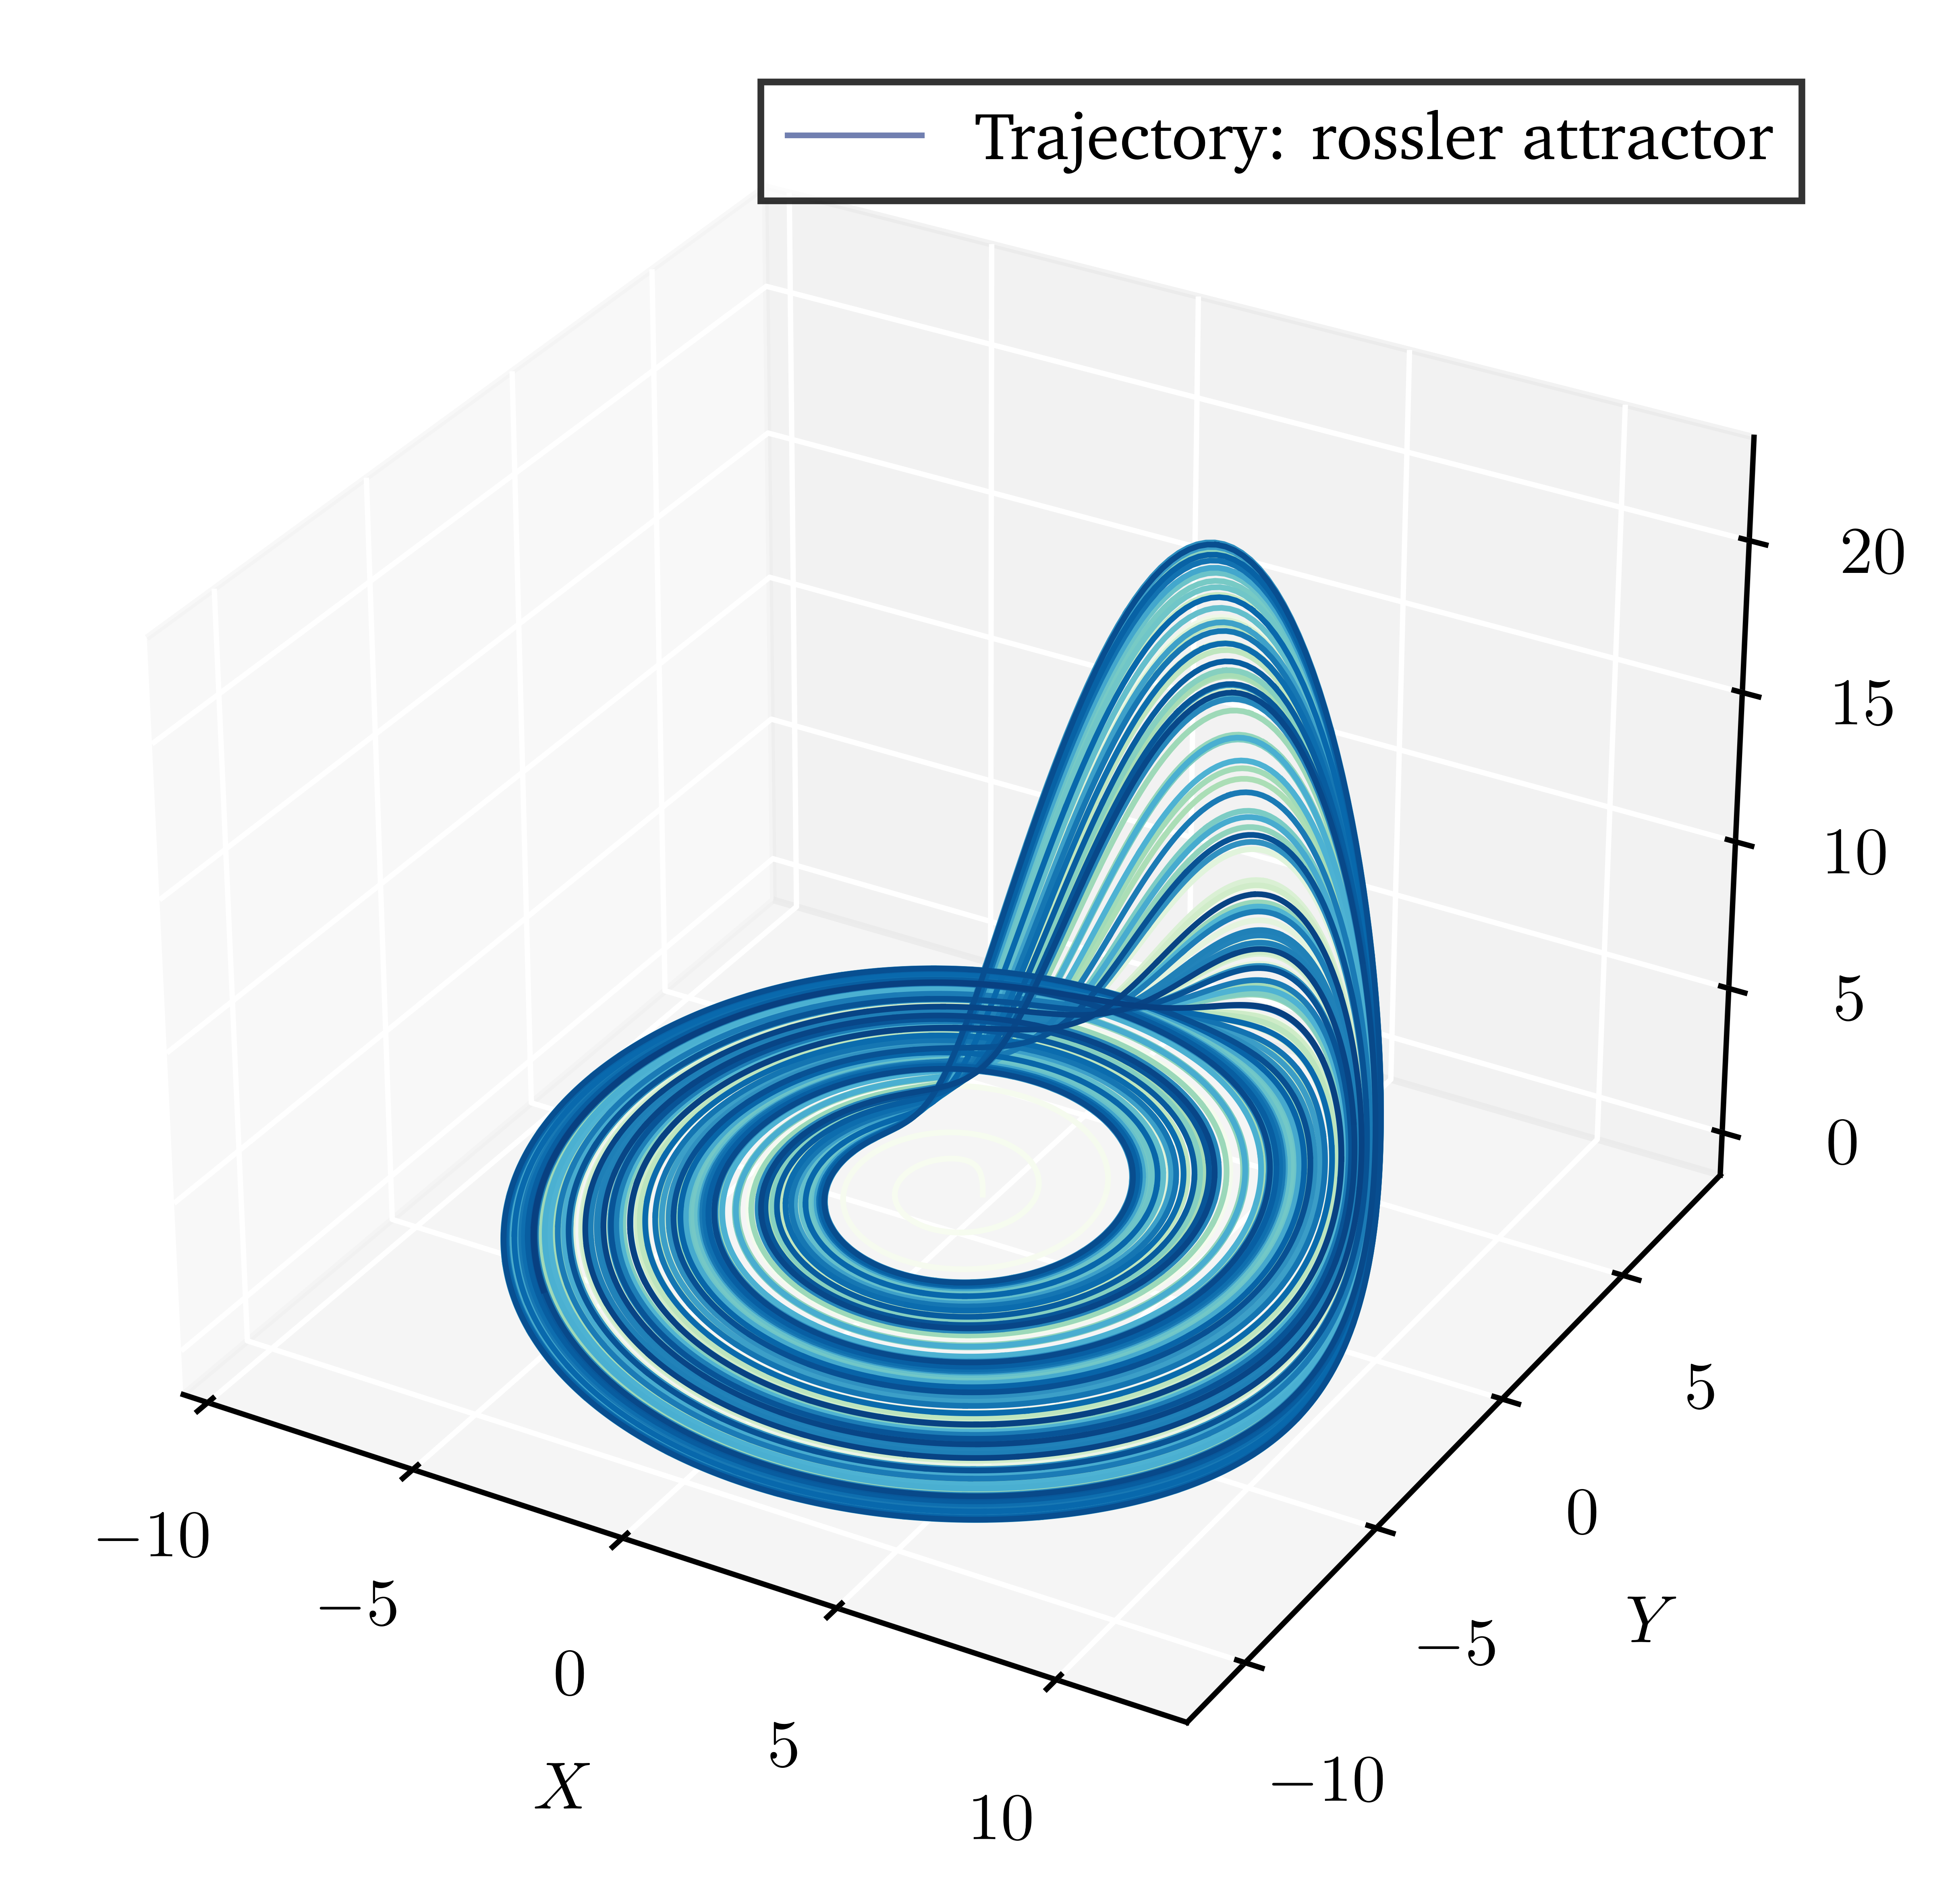
\includegraphics[scale=0.6]{figures/trajectories/traj_rossler.png}
        \column{0.45\linewidth}
        \begin{itemize}
            \setlength\itemsep{1em}
            \item[$\diamond$] Conditions initiales $\bm{r} = (1, 1, -1)$ \\
            \item[$\diamond$] Temps de $1000$ secondes
            \item[$\diamond$] Pas de $h = 0.001$
        \end{itemize}
    \end{columns}
\end{frame}

\begin{frame}
    \frametitle{Résultats - Trajectoires}
    \framesubtitle{Attracteur de Bouali}
    \begin{columns}
        \column{0.55\linewidth}
        \centering
        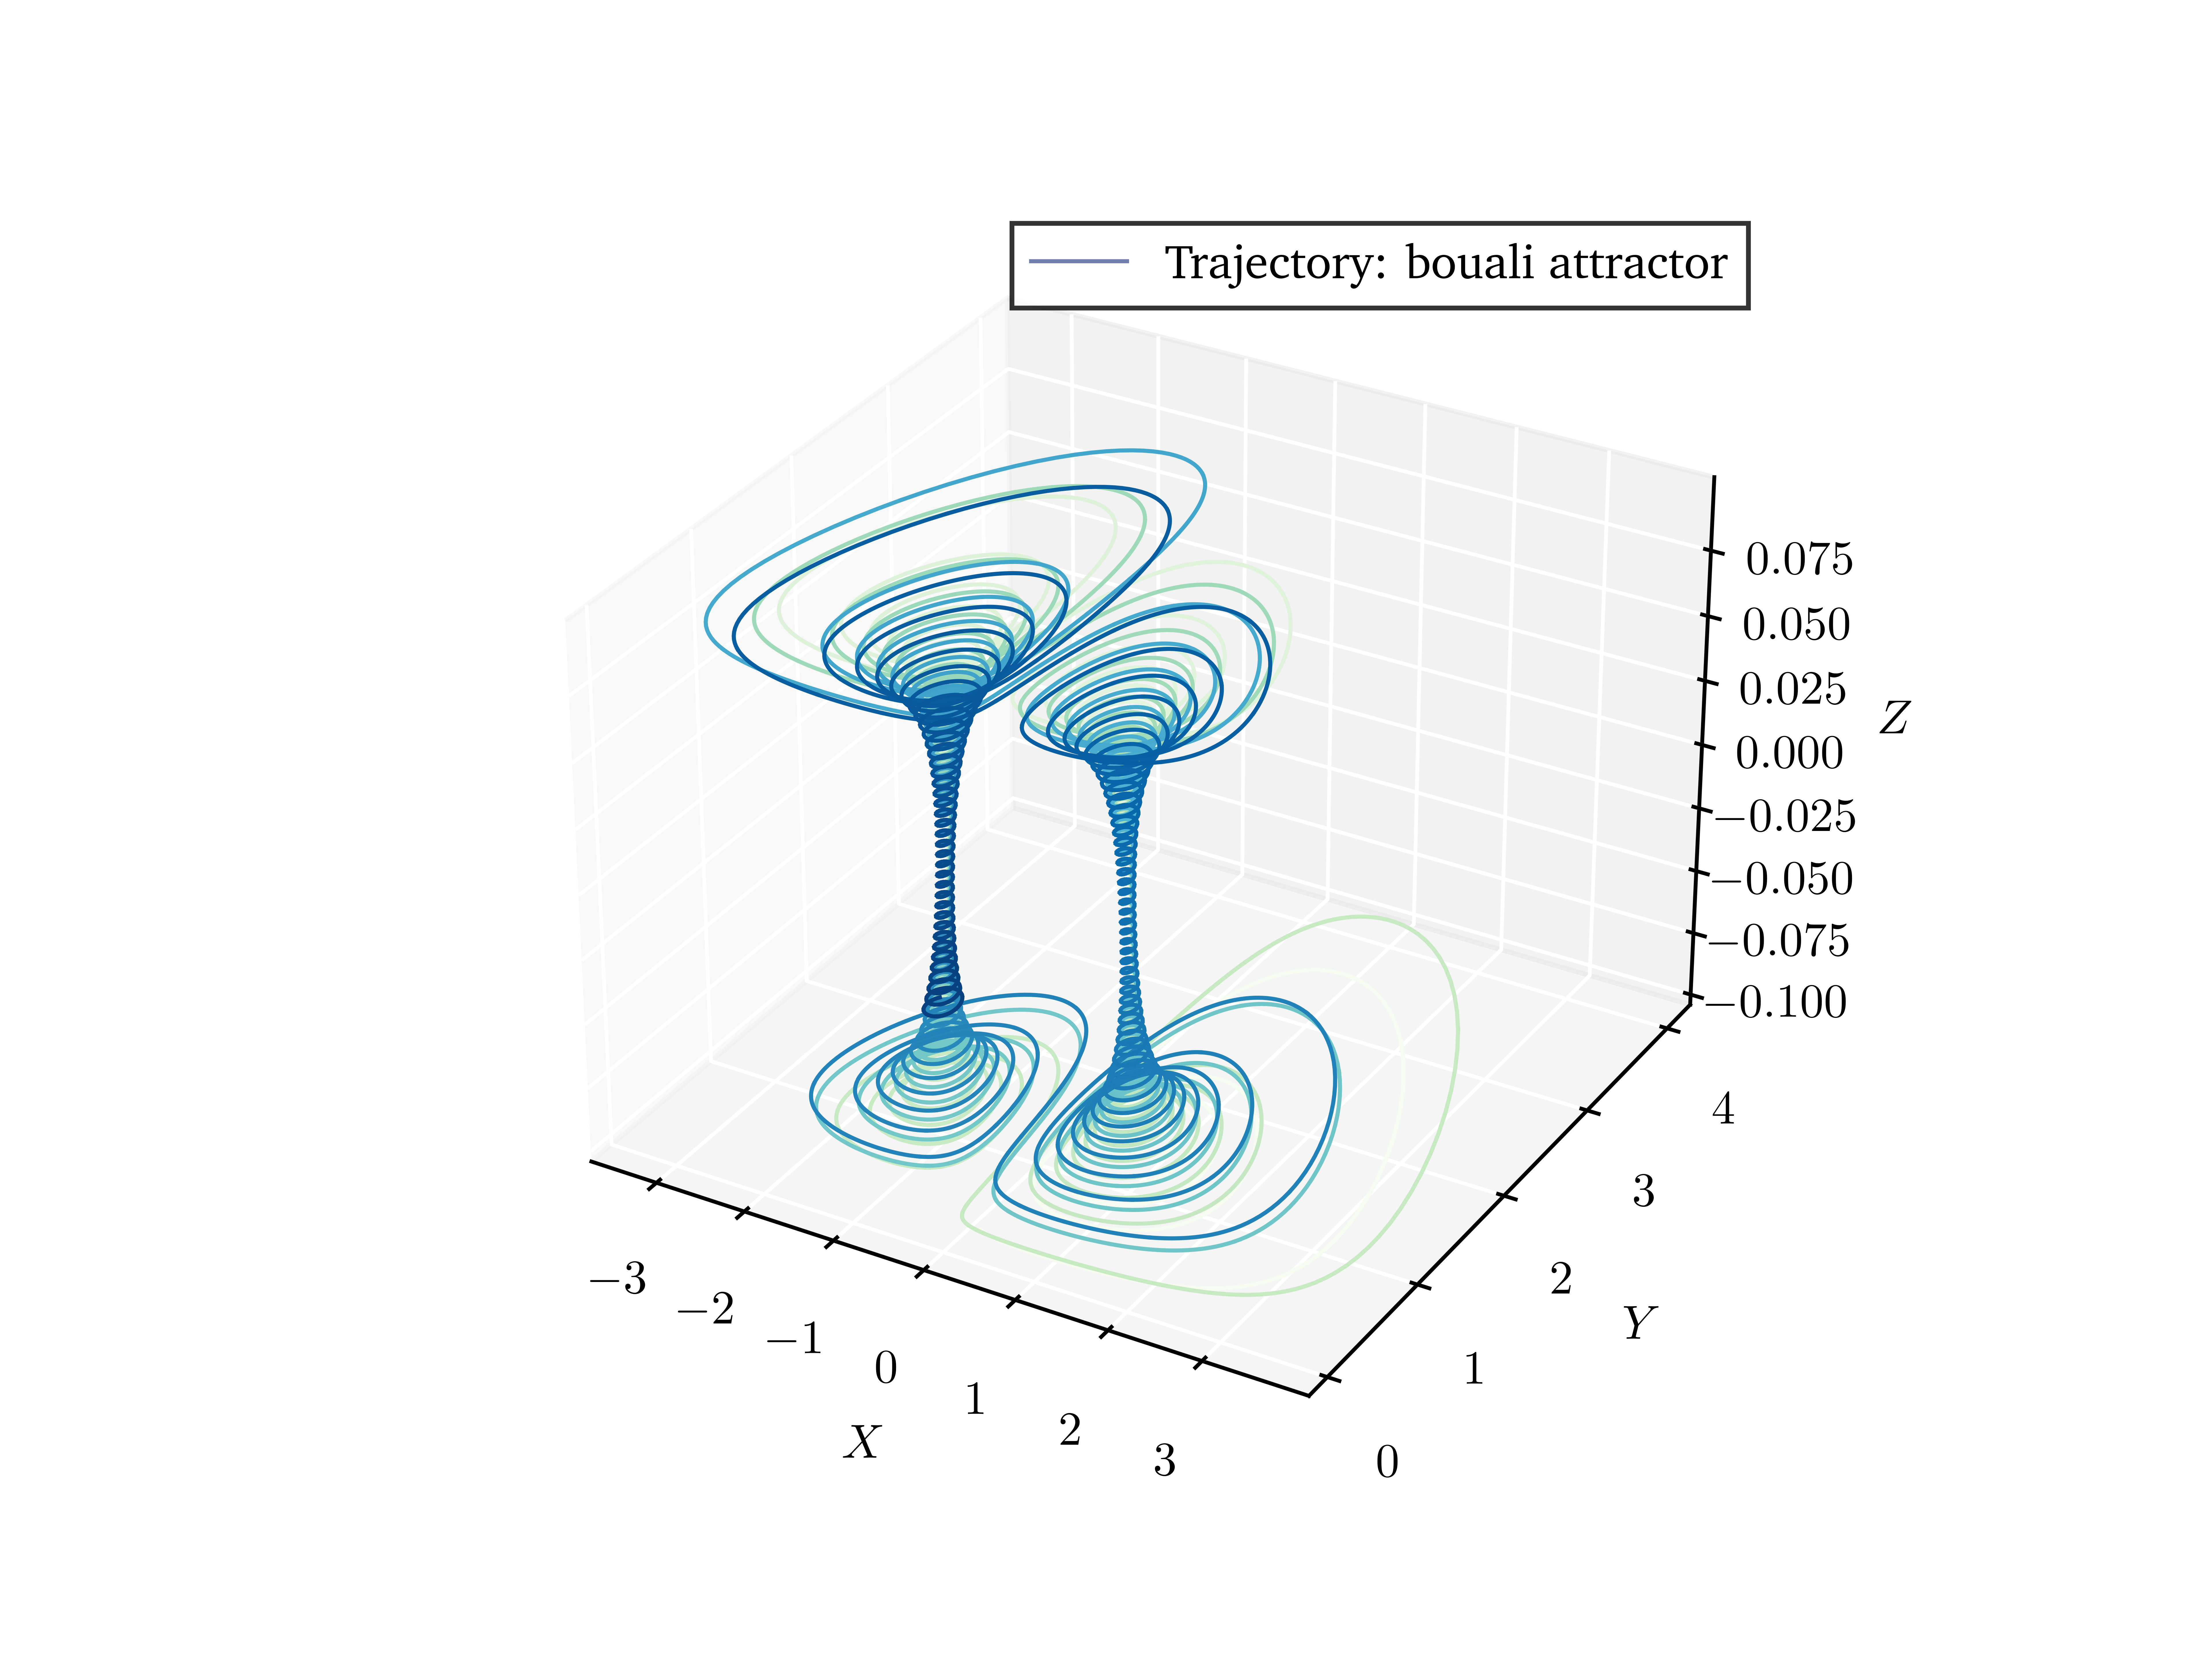
\includegraphics[scale=0.6]{figures/trajectories/traj_bouali.png}
        \column{0.45\linewidth}
        \begin{itemize}
            \setlength\itemsep{1em}
            \item[$\diamond$] Conditions initiales $\bm{r} = (0.2, 0.2, -0.08)$ \\
            \item[$\diamond$] Temps de $1000$ secondes
            \item[$\diamond$] Pas de $h = 0.001$
        \end{itemize}
    \end{columns}
\end{frame}

\begin{frame}
    \begin{center}
    \vspace{0.5cm}
    \boxed{
        Théorie - Spectre de Lyapunov \& Convergence
        }
    \end{center}
\end{frame}

\begin{frame}
    \frametitle{Théorie - Spectre de Lyapunov \& Convergence}
    \begin{columns}
        \column{0.55\linewidth}
        \centering
        \begin{figure}
            \begin{center}
                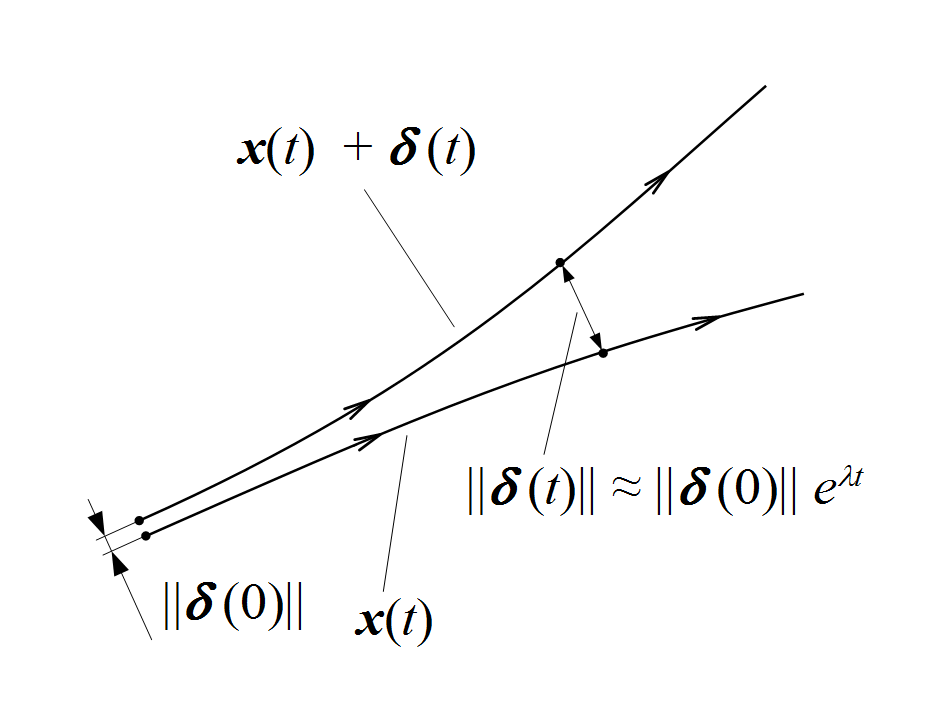
\includegraphics[scale=0.3]{figures/lyapunov_exponent.png}
            \end{center}
            \caption{Exposant de Lyapunov\footcite{LEswiki}.}
        \end{figure}
        \column{0.45\linewidth}
        \begin{itemize}
            \setlength\itemsep{1em}
            \item[$\diamond$] Le spectre de Lyapunov est de nature vectorielle
            \item[$\diamond$] Système dynamique de dimension $N$ $\implies\in\lambda_{i=1, 2\dots N}$ \\
        \end{itemize}
    \end{columns}
\end{frame}

\begin{frame}
    \frametitle{Théorie - Spectre de Lyapunov \& Convergence}
    Trois situations existent pour les exposants de Lyapunov $\lambda_j$:
    \vspace{0.5cm}
    \begin{itemize}
        \setlength\itemsep{1em}
        \item[$\diamond$] $\lambda_j > 0\implies$ signature chaotique
        \item[$\diamond$] $\lambda_j = 0\implies$ \textit{quasi-périodique}
        \item[$\diamond$] $\lambda_j < 0\implies$ convergence
    \end{itemize}
\end{frame}

\begin{frame}
    \frametitle{Théorie - Spectre de Lyapunov \& Convergence}
    L'équation qui permet d'obtenir l'exposant de Lyapunov dans la direction $j$ est
    \begin{align}
        \lambda_{j} = \lim_{n\to\infty}\frac{1}{n}\sum_{i = 0}^{n - 1}\ln(f^{(j)}(x_i))
    \end{align}
    \vspace{0.5cm}
    \begin{noteblock}{Note}
        Il est difficile de sommer un nombre infini numériquement. Quelles sont les solutions?
    \end{noteblock}
\end{frame}

\begin{frame}
    \begin{center}
    \vspace{0.5cm}
    \boxed{
        Méthodes numériques - Calculs matriciels \& Convergence
        }
    \end{center}
\end{frame}

\begin{frame}
    \frametitle{Méthodes numériques - Calculs matriciels \& Convergence}
    Numériquement, on procède de façon matricielle $\to$ $J$
    \vspace{0.5cm}
    \begin{defblock}{Définition: Matrice Jacobienne}
        Les éléments de la matrice jacobienne sont donnés par
        \begin{align}
            J_{ij} = \frac{\partial f_i}{\partial x_j},
        \end{align}
        où $f_i$ est l'équation $i$ et $x_j$ la variable de dérivation.
    \end{defblock}
\end{frame}

\begin{frame}
    \frametitle{Méthodes numériques - Calculs matriciels \& Convergence}
    Évolution volumique d'une sphère unitaire $U_{3x3}$ $\to$ taux de variation donnés par $J$. L'algorithme est qualitativement \pause
    \vspace{0.5cm}
    \begin{itemize}
        \setlength\itemsep{1em}
        \item[$\diamond$] Position sur la trajectoire $\bm{r}(t_n)$ \pause
        \item[$\diamond$] Évaluation de $J$ en ce point \pause
        \item[$\diamond$] Taux de contraction/expansion ($J\cdot U$) \pause
        \item[$\diamond$] Extraction du spectre de Lyapunov ($Q\cdot R$) \pause
        \item[$\diamond$] Mise à jours des perturbations de l'espace des phases au temps $t_n$
    \end{itemize}
\end{frame}

\begin{frame}
    \frametitle{Méthodes numériques - Calculs matriciels \& Convergence}
    \begin{columns}
        \column{0.5\linewidth}
        \centering
        \begin{figure}
            \begin{center}
                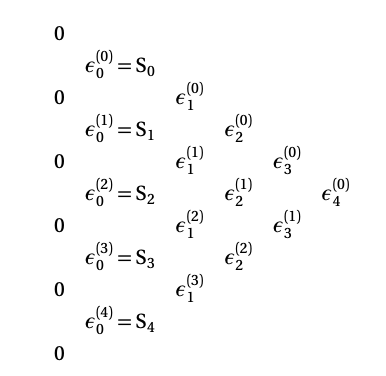
\includegraphics[scale=0.4]{figures/epsilon_tri_array.png}
            \end{center}
            \caption{\parencite{SENECH}.}
        \end{figure}
        \column{0.5\linewidth}
        Convergence du spectre de Lyapunov dans la limite $t\to\infty$ grâce à l'algorithme \textit{epsilon}
    \end{columns}
\end{frame}

\begin{frame}
    \begin{center}
    \vspace{0.5cm}
        \boxed{
        Résultats - Spectre de Lyapunov
        }
    \end{center}
\end{frame}

\begin{frame}
    \frametitle{Résultats - Spectre de Lyapunov}
    \framesubtitle{Attracteur de Lorenz}
    Simulation pour 100 secondes avec $10^4$ points et $\bm{r}_0 = (1, 0, -1)$
    \vspace{1cm}
    \begin{columns}
        \column{0.5\linewidth}
        \centering
        \includegraphics[scale=0.4]{figures/lyapunovs/lyap_lorenz.png}
        \column{0.5\linewidth}
        \includegraphics[scale=0.4]{figures/lyapunovs/lyap_lorenz_zoom.png}
    \end{columns}
\end{frame}

\begin{frame}
    \frametitle{Résultats - Spectre de Lyapunov}
    \framesubtitle{Attracteur de Rössler}
    Simulation pour 500 secondes avec $10^5$ points et $\bm{r}_0 = (1, 1, -1)$
    \vspace{1cm}
    \begin{columns}
        \column{0.5\linewidth}
        \centering
        \includegraphics[scale=0.4]{figures/lyapunovs/lyap_rossler.png}
        \column{0.5\linewidth}
        \includegraphics[scale=0.4]{figures/lyapunovs/lyap_rossler_zoom.png}
    \end{columns}
\end{frame}

\begin{frame}
    \frametitle{Résultats - Spectre de Lyapunov}
    \framesubtitle{Attracteur de Bouali}
    Simulation pour 500 secondes avec $10^5$ points et $\bm{r}_0 = (0.2, 0.2, -0.08)$
    \vspace{1cm}
    \begin{columns}
        \column{0.5\linewidth}
        \centering
        \includegraphics[scale=0.4]{figures/lyapunovs/lyap_bouali.png}
        \column{0.5\linewidth}
        \includegraphics[scale=0.4]{figures/lyapunovs/lyap_bouali_zoom.png}
    \end{columns}
\end{frame}


    \section{Résultats} \label{sec: resultats}

\subsection{Trajectoires} \label{subsec: res_trajectories}
    Soit les figures \ref{fig: traj_lorenz}, \ref{fig: traj_rossler} et
    \ref{fig: traj_bouali} qui présentent les résultats pour la simulation des
    attracteurs (Lorenz, Rössler et Bouali) définis mathématiquement dans la
    section \fullref{sec: theory}. On voit sur lesdites figures la trajectoires
    d'une particule de masse unité dans les systèmes dynamiques dissipatifs
    représentés par les différents attracteurs. Étonnement, les trajectoires
    montrées sur ces figures ne semble pas du tout chaotiques, et se
    rapprochent d'arrangements très bien organisés voir même prédictibles. Une
    fois de plus, la subtilité réside dans la sensibilité de ces systèmes aux
    conditions initiales. Il est d'ailleurs à noter que ces figures sont des
    trajectoires qui proviennent d'\textbf{une seule} position initiale à
    chaque fois. Pour voir à quel point ces attracteurs sont chaotiques ou non,
    nous devrions exécuter la simulation pour une multitude de coordonnées
    initiales et ainsi observer la divergence très précoce entre les solutions.
    Un bon indicateur de signature chaotique est le spectre de Lyapunov et
    c'est pourquoi nous allons analyser ce spectre en utilisant les mêmes
    trajectoires attractives. \\

    Il est également intéressant d'observer sur les figures
    \ref{fig: traj_lorenz}, \ref{fig: traj_rossler} et \ref{fig: traj_bouali}
    que le théorème d'unicité des solutions d'équations différentielles
    ordinaires est vérifié \cite{uniqueness}. On observe effectivement aucun
    croisement dans les trajectoires obtenues.

\subsection{Spectre de Lyapunov} \label{subsec: res_lyapunov}
    Considérons les figures \ref{fig : lyaps_lorenz},
    \ref{fig : lyaps_rossler} et \ref{fig : lyaps_bouali}, sur lesquelles ont
    observe le calcul du spectre de Lyapunov en fonction du temps pour les
    trajectoires attractives discutées dans la section
    \fullref{subsec: res_trajectories}. Il est intéressant d'observer la
    précieuse utilisation de l'algorithme de convergence epsilon introduit dans
    la section \fullref{subsec: convergence}. La convergence est pertinente et
    permet bien d'identifier le comportement à long terme
    ($\lim_{t\to\infty}\lambda_i(t)$) du spectre de Lyapunov pour la
    trajectoire des attracteurs étudiés. \\

    On remarque premièrement, pour tous les attracteurs, que l'exposant de
    Lyapunov maximal $\lambda_1$ est positif. Comme introduit dans la section
    \fullref{subsec: lyapunov}, il s'agit-là d'une signature typique de chaos.
    Mathématiquement, cela signifie que dans la direction associée à l'exposant
    $\lambda_1$ deux trajectoires voisines divergent exponentiellement
    rapidement dans le temps et donc que de toutes petites perturbations
    peuvent mener à des trajectoires très différentes. On peut ici faire un
    lien avec la contraction/expansion de l'espace des phases modélisée par
    l'évolution du volume de la sphère unitaire $U$ vis-à-vis du signe obtenu
    pour les composantes du spectre de Lyapunov. \\

    Ensuite, on remarque que dans les résultats obtenus, deux des trois
    exposants sont négatifs. Cela signifie logiquement que deux trajectoires
    voisines tendent à converger au sein de l'attracteur et demeurer près l'une
    de l'autre. Physiquement, on peut aussi dire que des exposants négatifs
    indiquent que les systèmes étudiés sont dissipatifs (perdent de l'énergie
    au cours du temps) et donc qu'il est normal d'observer la convergence de
    certaines trajectoires comme par exemple lorsque l'on étudie un oscillateur
    harmonique amorti. \\

    Finalement, on voit que certains des exposants de Lyapunov sont nuls. Ces
    derniers n'impliquent pas de comportement chaotique particuliers. On peut
    conclure que mathématiquement, une perturbation d'une trajectoire ayant un
    exposant de Lyapunov nul peut se voir diverger mais seulement de façon
    logarithmique. On appelle ce phénomène:
    \textit{comportement quasi-périodique}.

\onecolumngrid
\vspace{2cm}

    \begin{figure}[h!]
        \centering
        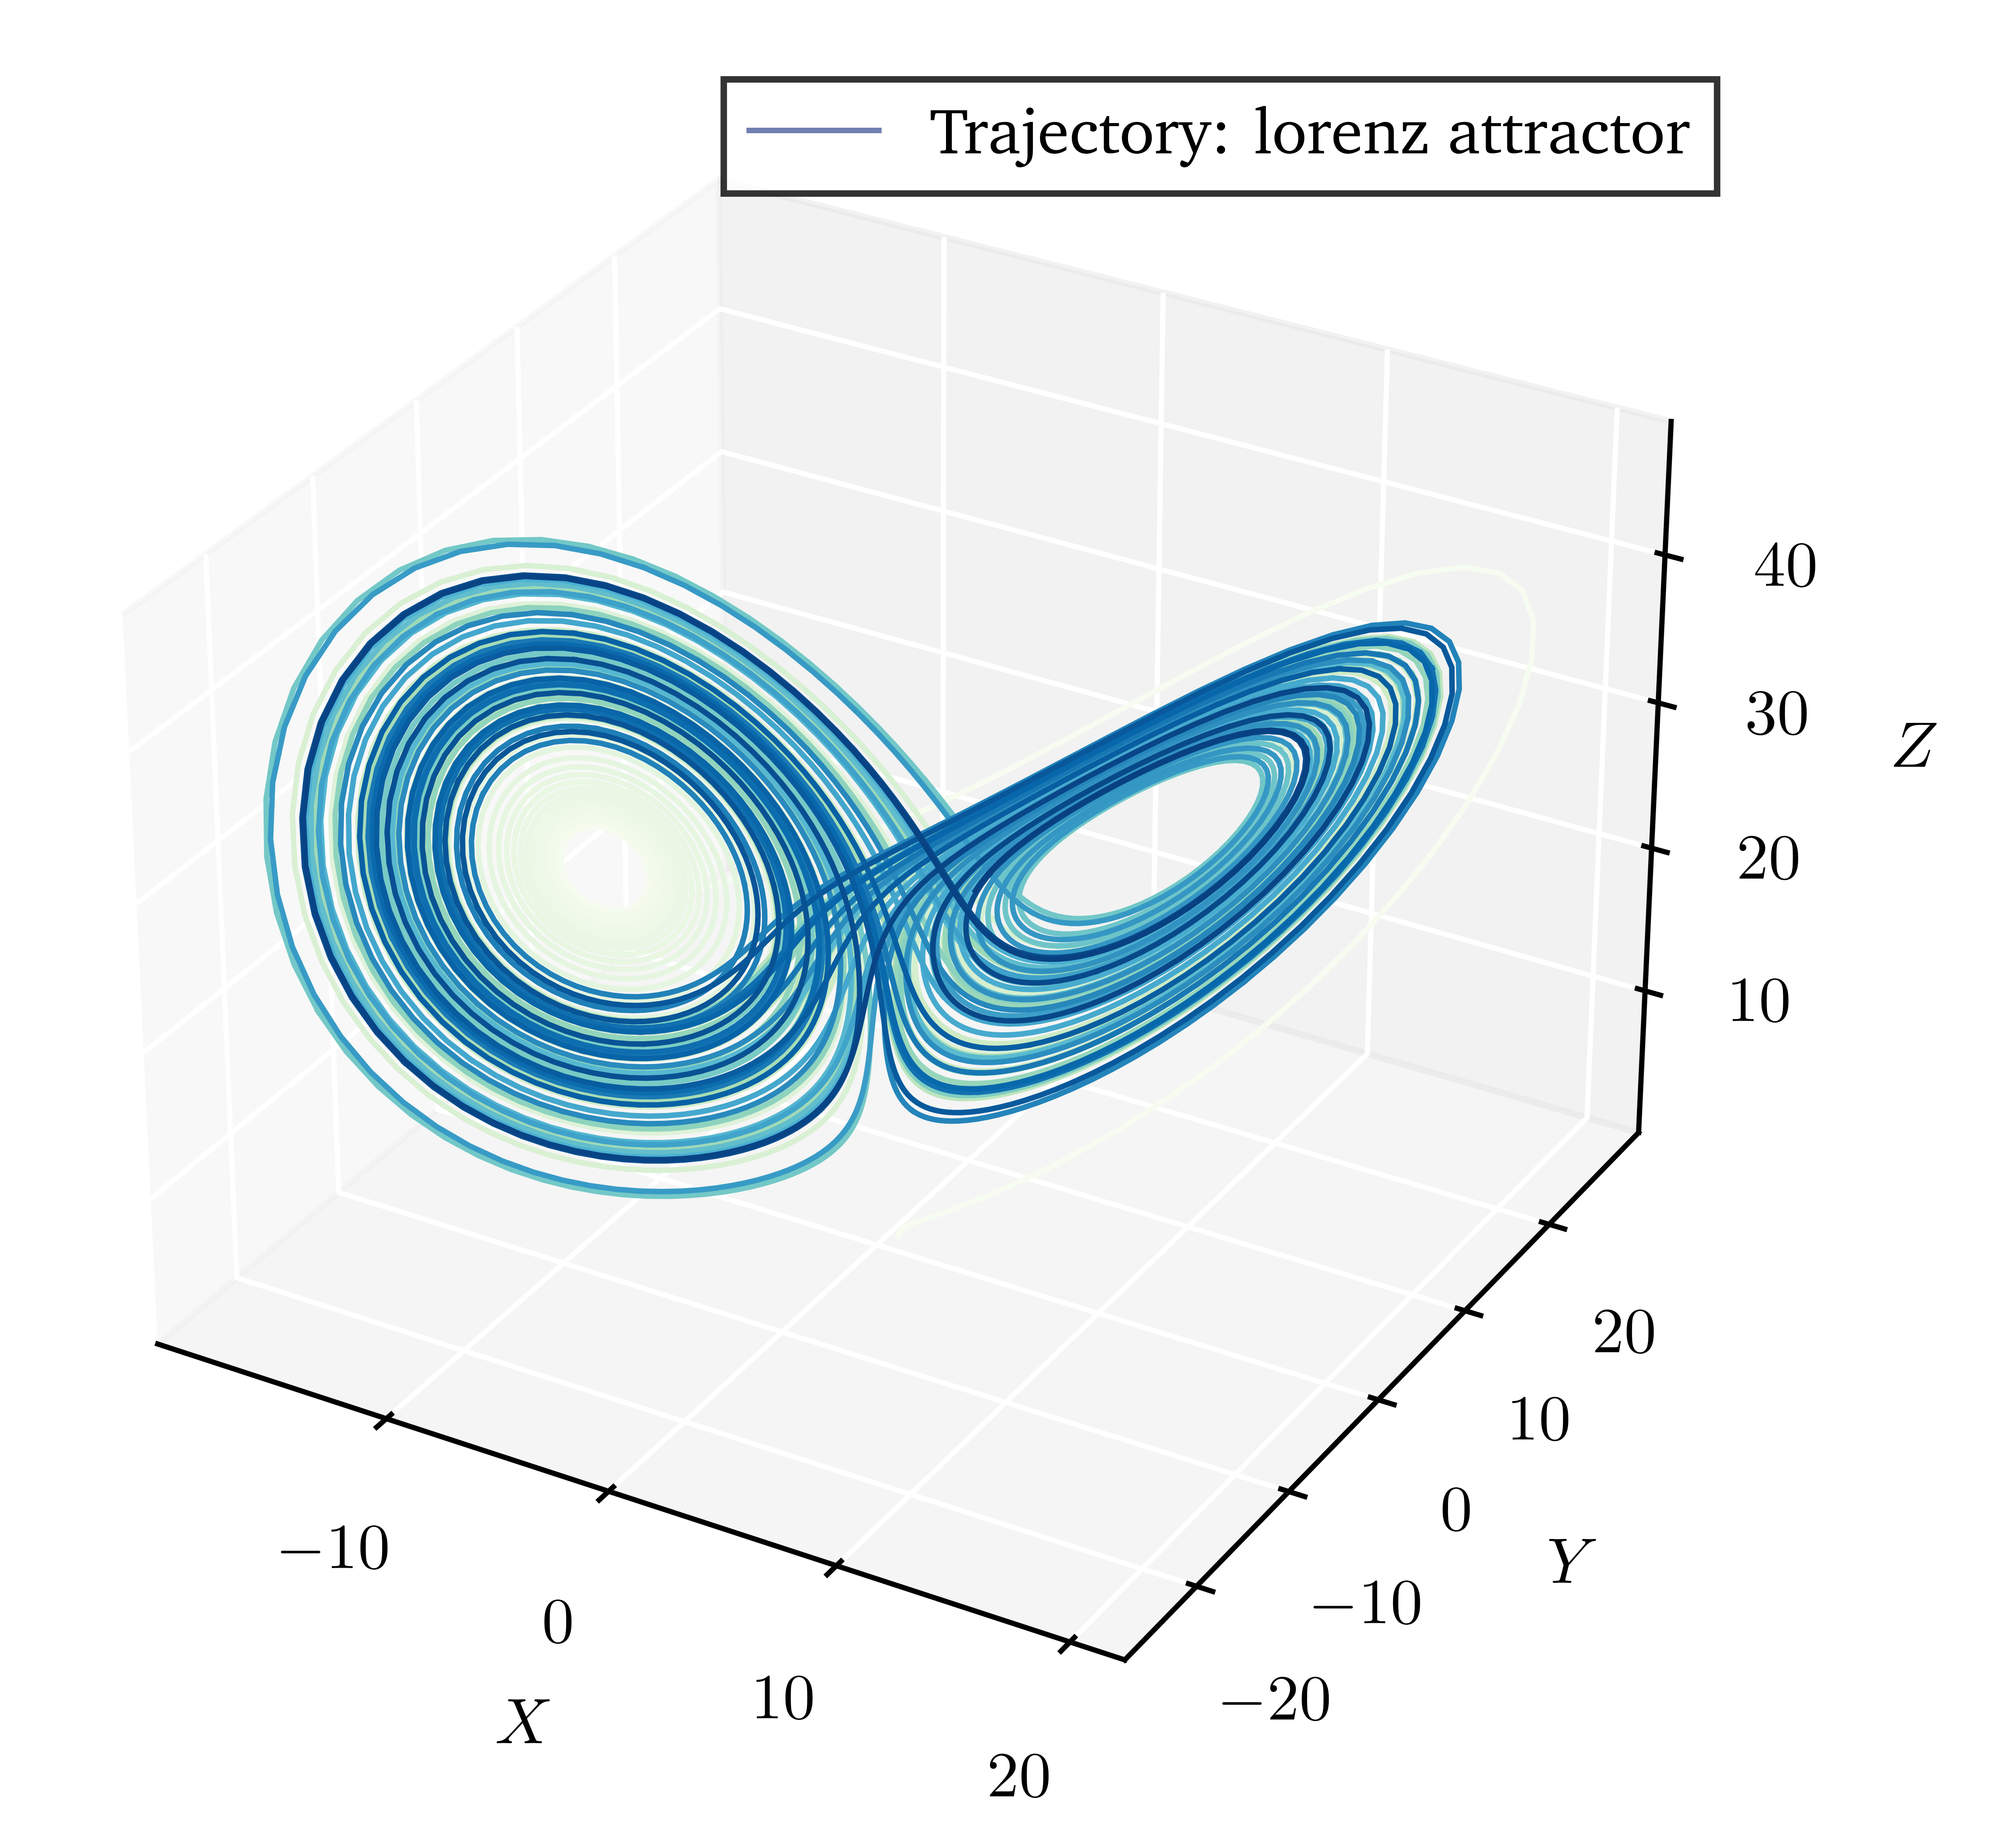
\includegraphics[scale=0.6]{figs/trajectories/traj_lorenz.png}
        \caption{Trajectoire obtenue pour la simulation d'une particule de
        masse unité dans le bassin d'attraction de l'attracteur de Lorenz ayant
    comme position initiale $\bm{r}_0 = (1, 0, -1)$ ainsi que pour un temps de
100 secondes avec un pas de $h = 0.01$.}
        \label{fig: traj_lorenz}
    \end{figure}
    \vspace{1cm}
    \begin{figure}[h!]
        \centering
        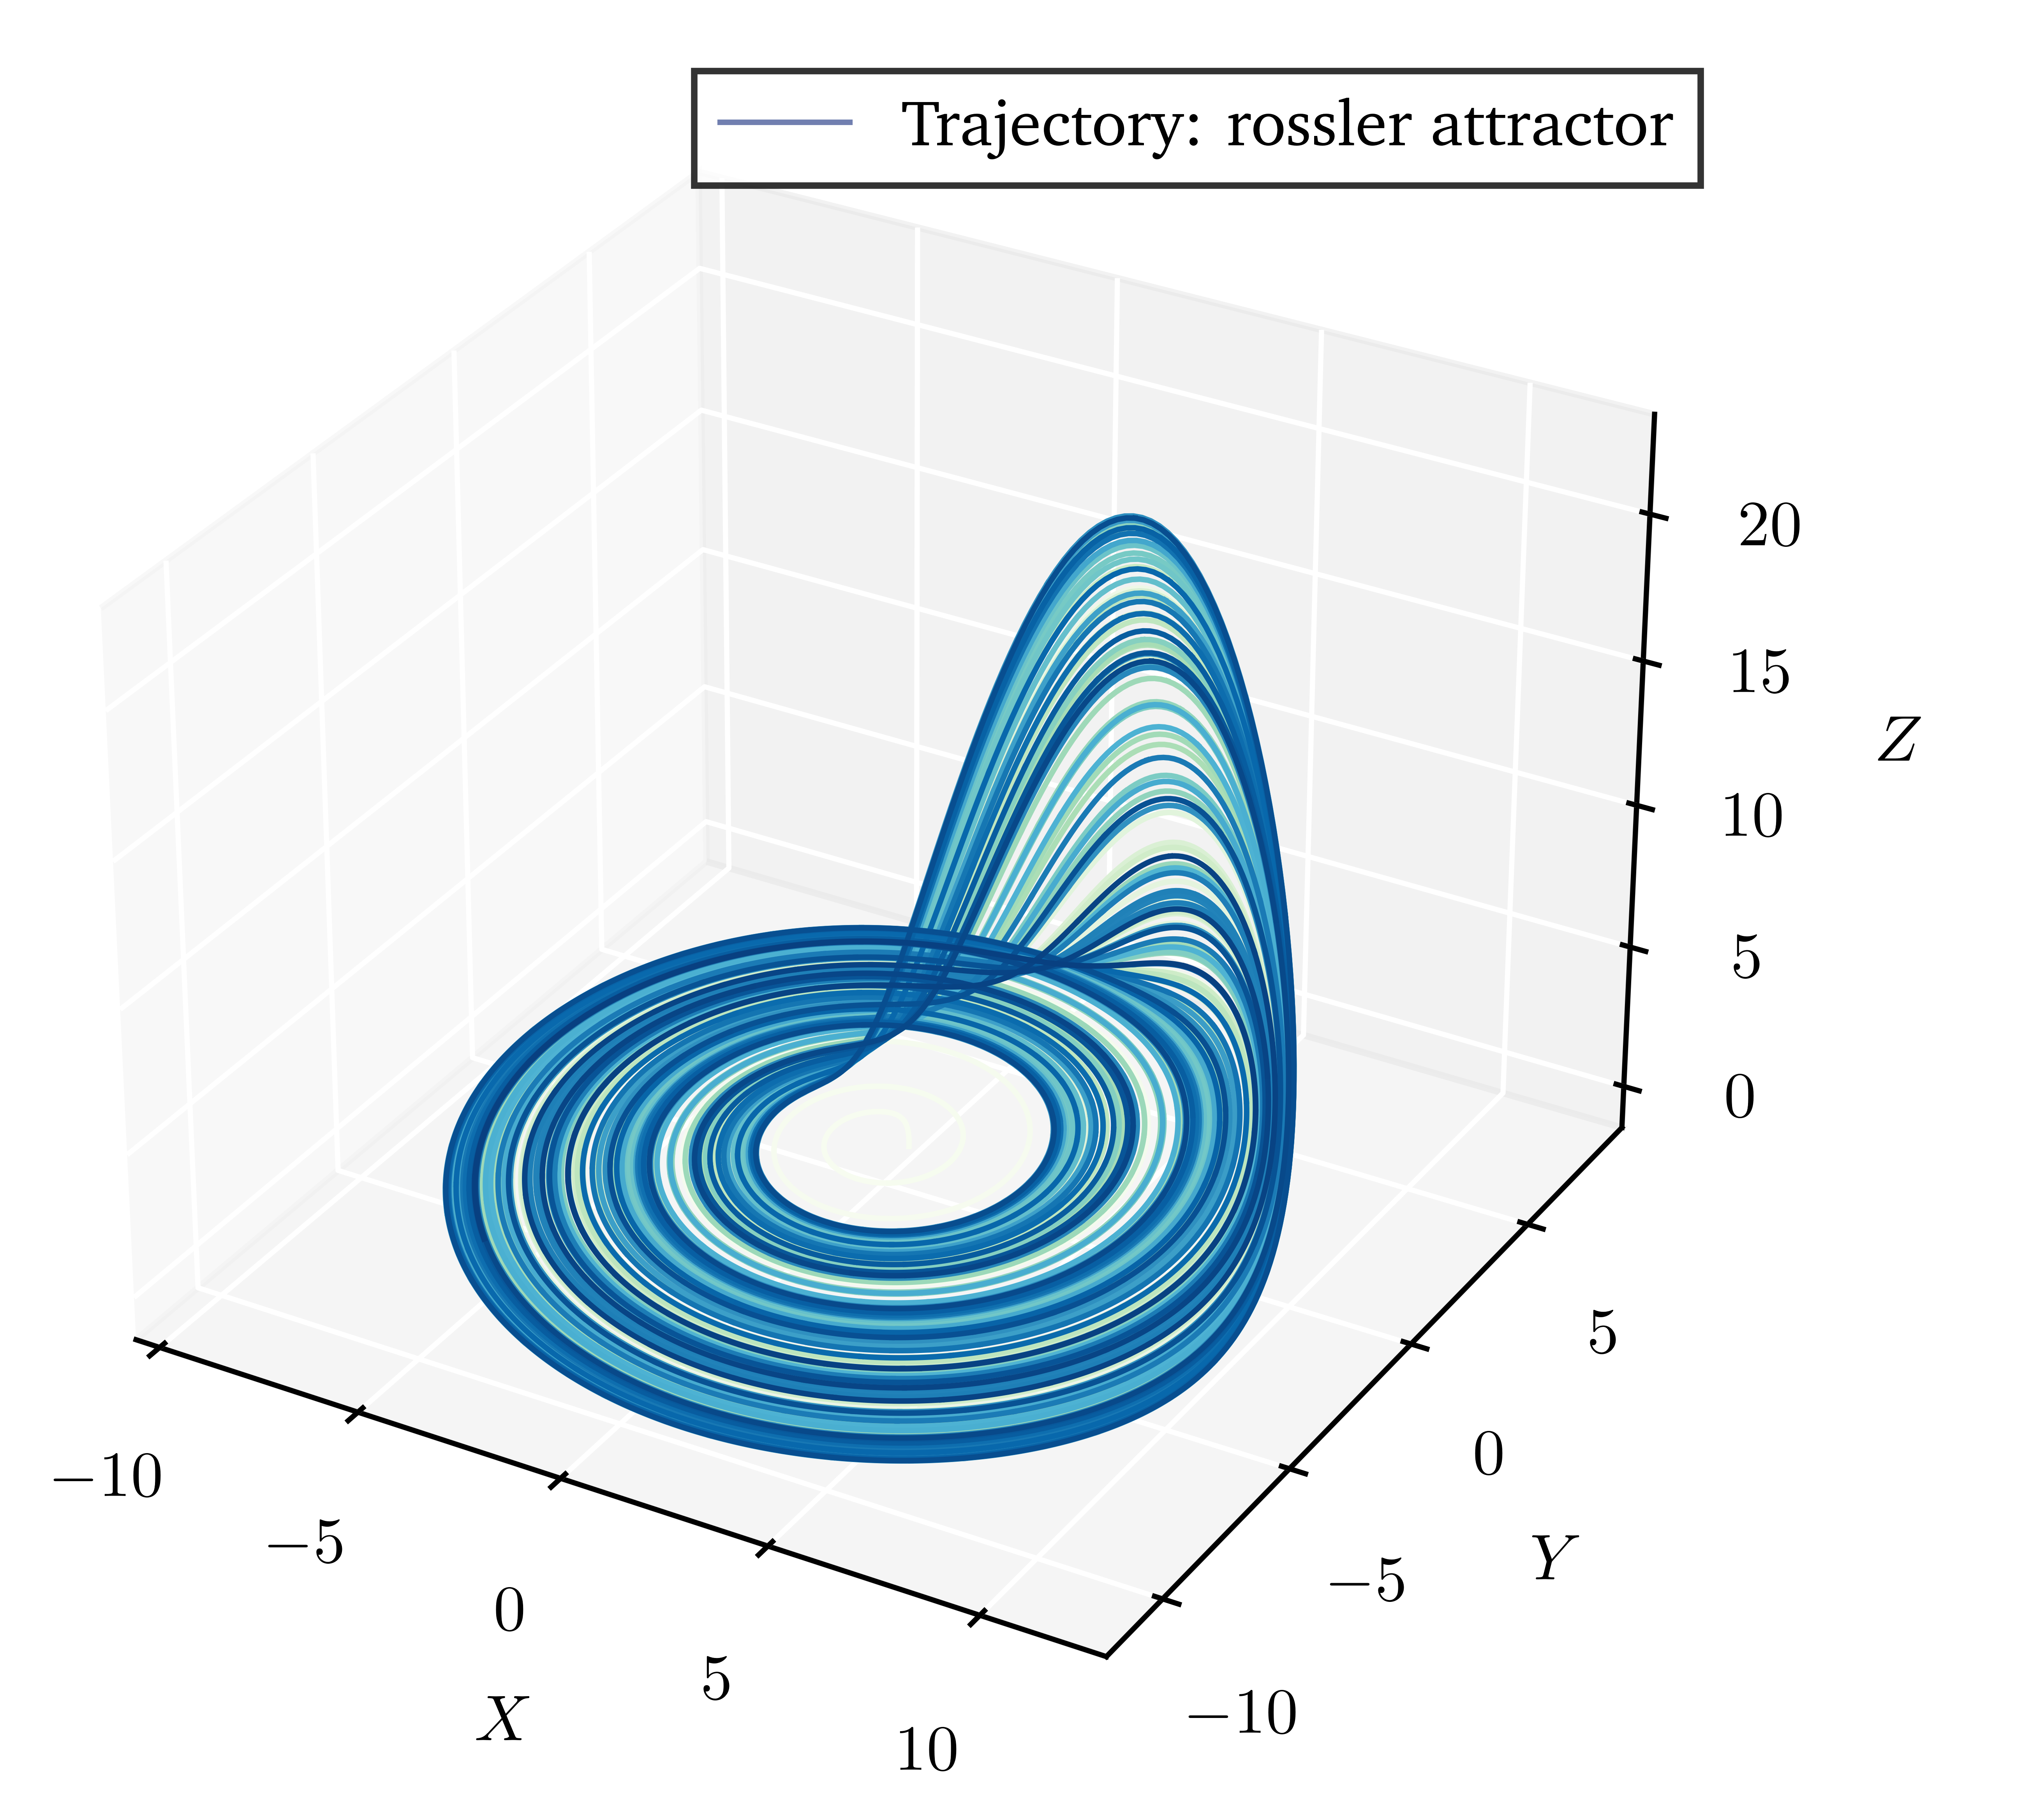
\includegraphics[scale=0.6]{figs/trajectories/traj_rossler.png}
        \caption{Trajectoire obtenue pour la simulation d'une particule de
        masse unité dans le bassin d'attraction de l'attracteur de Rössler ayant
    comme position initiale $\bm{r}_0 = (1, 1, -1)$ ainsi que pour un temps de
1000 secondes avec un pas de $h = 0.001$.}
        \label{fig: traj_rossler}
    \end{figure}

\clearpage

    \begin{figure}[h!]
        \centering
        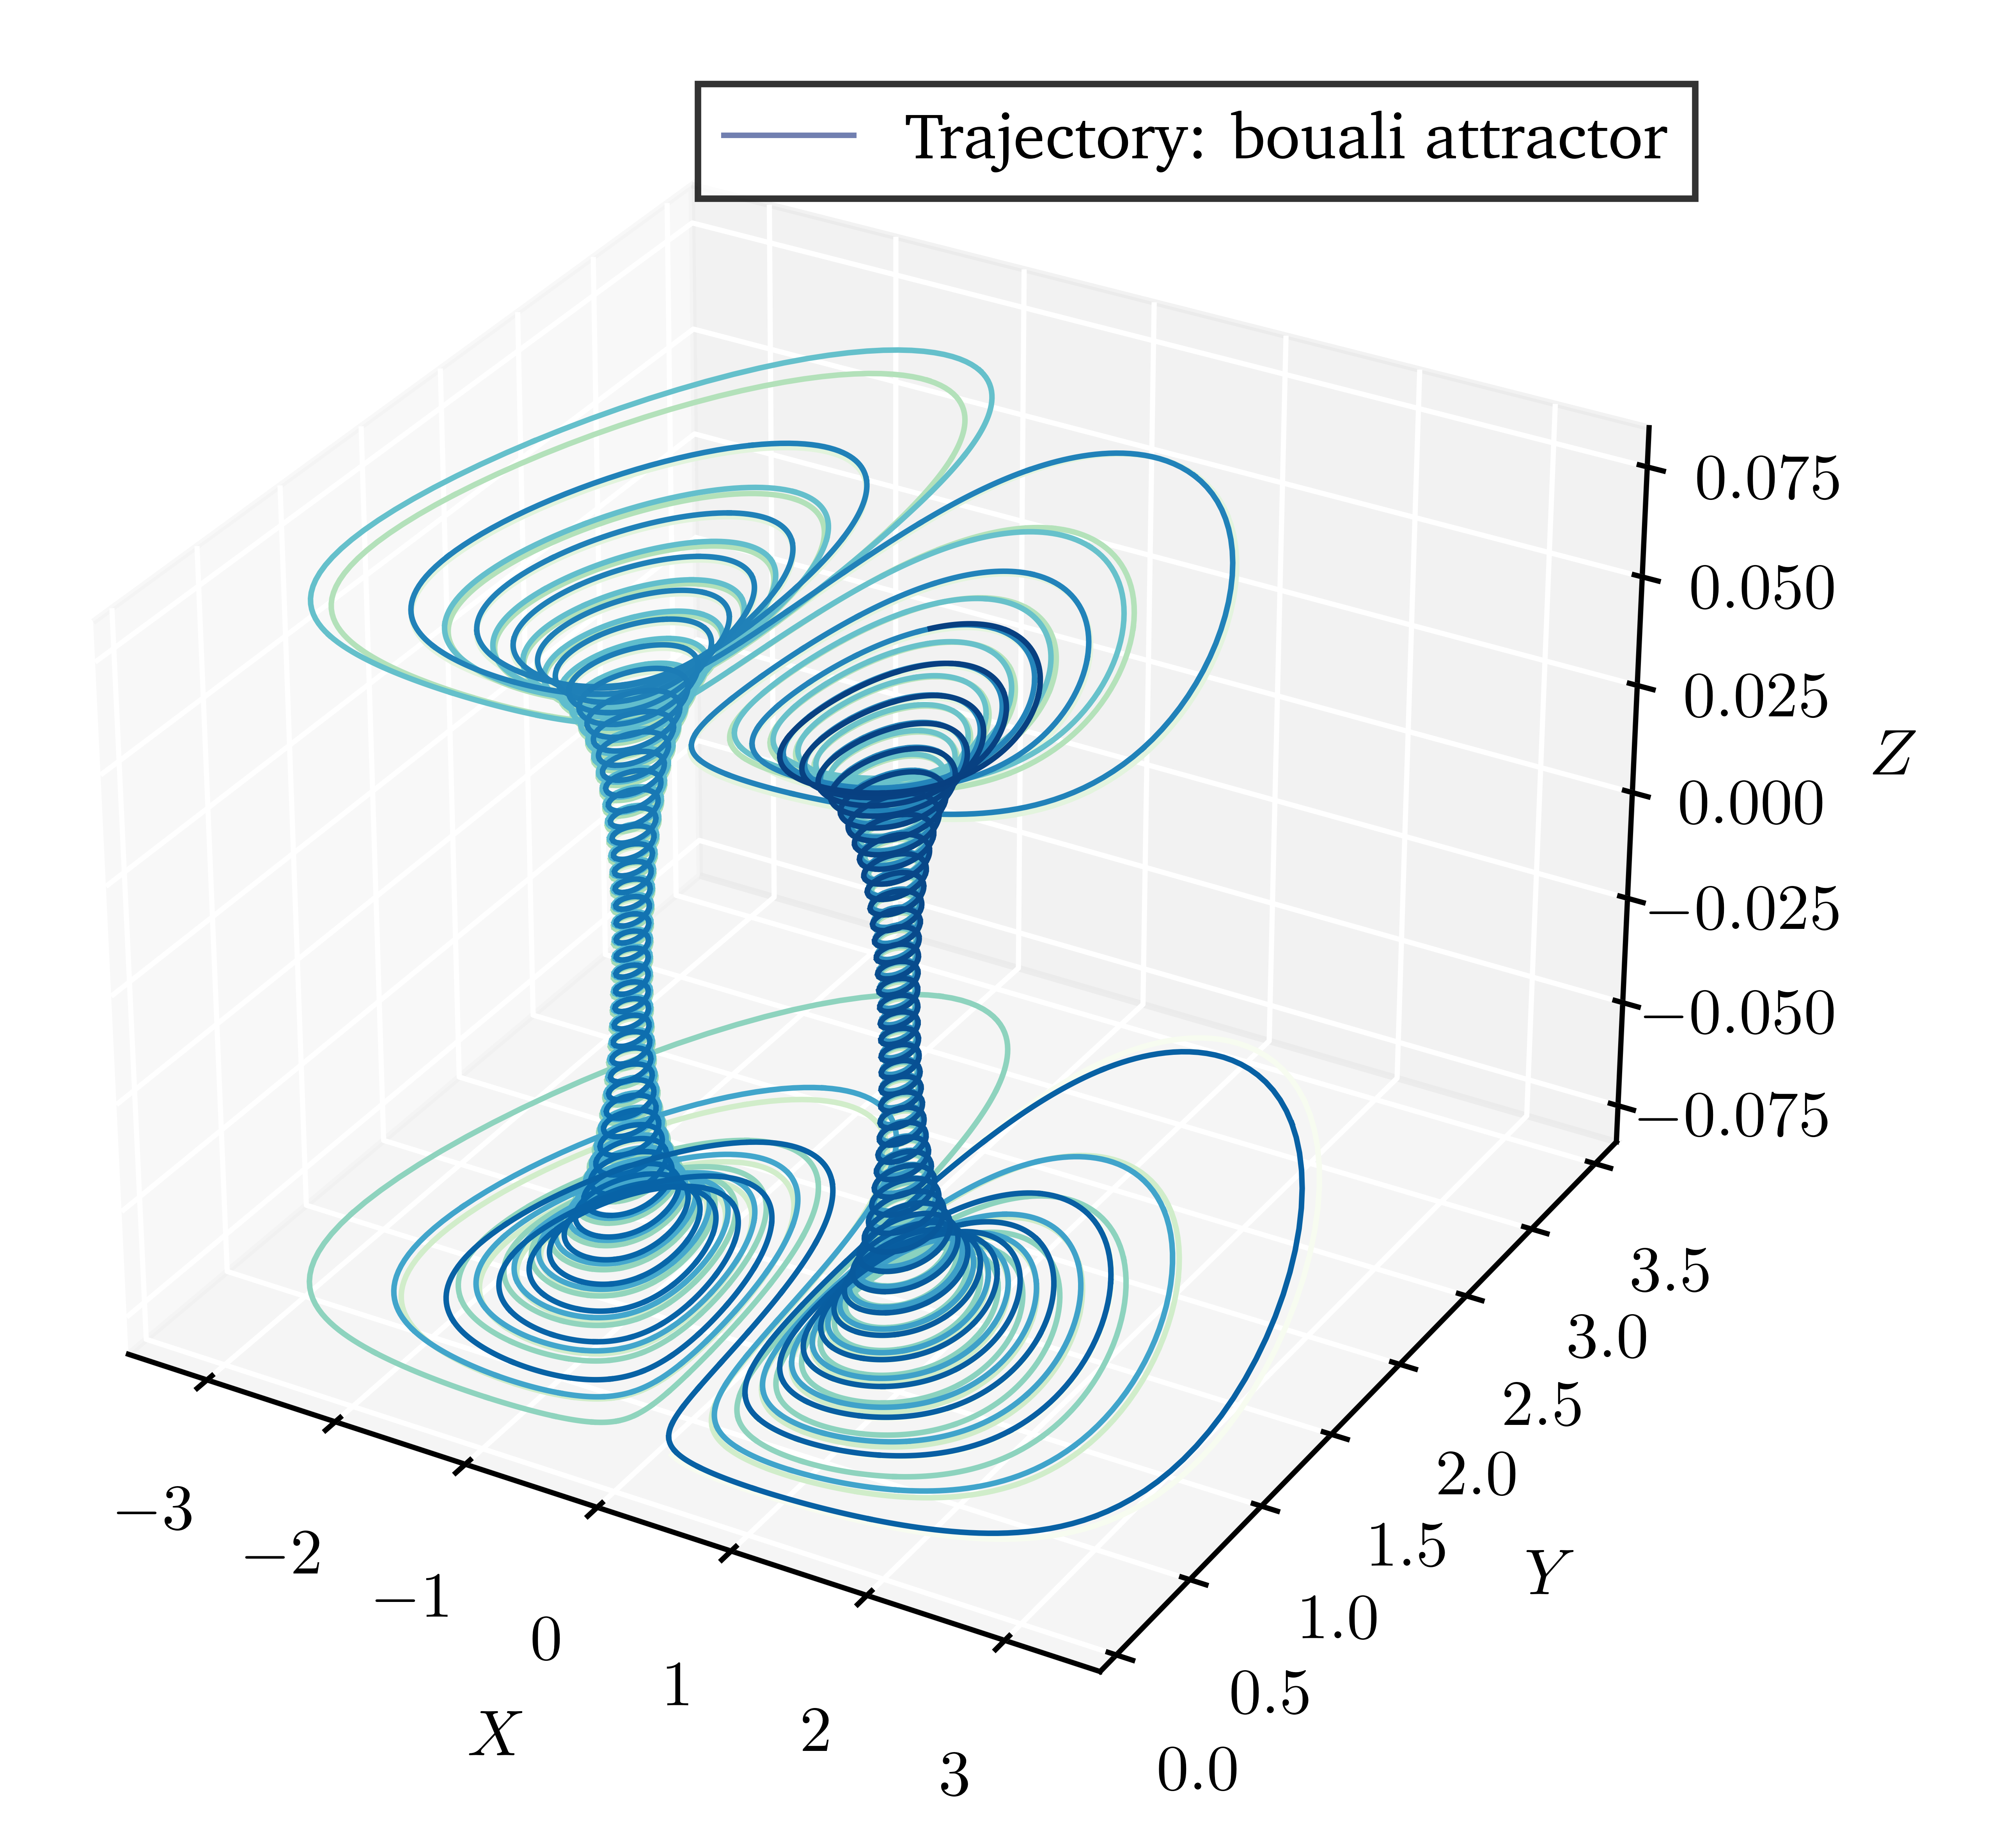
\includegraphics[scale=0.6]{figs/trajectories/traj_bouali.png}
        \caption{Trajectoire obtenue pour la simulation d'une particule de
        masse unité dans le bassin d'attraction de l'attracteur de Bouali ayant
    comme position initiale $\bm{r}_0 = (0.2, 0.2, -0.08)$ ainsi que pour un
temps de 1000 secondes avec un pas de $h = 0.001$.}
        \label{fig: traj_bouali}
    \end{figure}

    \begin{figure}[h!]
        \centering
        \begin{minipage}{0.49\textwidth}
          \centering
          \includegraphics[scale = 0.4]{figs/lyapunovs/lyap_lorenz.png}
          \subcaption{}
          \label{fig: lyap_lorenz}
        \end{minipage}
        \begin{minipage}{0.49\textwidth}
          \centering
          \includegraphics[scale = 0.4]{figs/lyapunovs/lyap_lorenz_zoom.png}
          \subcaption{}
          \label{fig: lyap_lorenz_zoom}
        \end{minipage}
        \caption{Spectre de Lyapunov ($\lambda_i\forall i\in\{1, 2, 3\}$) dans
        la simulation de l'attracteur de Lorenz. (a) Spectre complet. (b) Mise
    en évidence du comportement pour les exposants $\lambda_1$ et $\lambda_2$
étant donnée la superposition et le bruit.}
        \label{fig : lyaps_lorenz}
    \end{figure}

    \begin{figure}[h!]
        \centering
        \begin{minipage}{0.49\textwidth}
          \centering
          \includegraphics[scale = 0.4]{figs/lyapunovs/lyap_rossler.png}
          \subcaption{}
          \label{fig: lyap_rossler}
        \end{minipage}
        \begin{minipage}{0.49\textwidth}
          \centering
          \includegraphics[scale = 0.4]{figs/lyapunovs/lyap_rossler_zoom.png}
          \subcaption{}
          \label{fig: lyap_rossler_zoom}
        \end{minipage}
        \caption{Spectre de Lyapunov ($\lambda_i\forall i\in\{1, 2, 3\}$) dans
        la simulation de l'attracteur de Rössler. (a) Spectre complet. (b) Mise
    en évidence du comportement pour les exposants $\lambda_1$ et $\lambda_2$
étant donnée la superposition et le bruit.}
        \label{fig : lyaps_rossler}
    \end{figure}

    \clearpage

    \begin{figure}[h!]
        \centering
        \begin{minipage}{0.49\textwidth}
          \centering
          \includegraphics[scale = 0.4]{figs/lyapunovs/lyap_bouali.png}
          \subcaption{}
          \label{fig: lyap_bouali}
        \end{minipage}
        \begin{minipage}{0.49\textwidth}
          \centering
          \includegraphics[scale = 0.4]{figs/lyapunovs/lyap_bouali_zoom.png}
          \subcaption{}
          \label{fig: lyap_bouali_zoom}
        \end{minipage}
        \caption{Spectre de Lyapunov ($\lambda_i\forall i\in\{1, 2, 3\}$) dans
        la simulation de l'attracteur de Bouali. (a) Spectre complet. (b) Mise
    en évidence du comportement pour les exposants $\lambda_1$, $\lambda_2$ et
$\lambda_3$ étant donnée la superposition et le bruit.}
        \label{fig : lyaps_bouali}
    \end{figure}

\twocolumngrid


    \section{Conclusion}

\begin{frame}
    \begin{center}
    \vspace{0.5cm}
    \boxed{
        Conclusion
    }
    \end{center}
\end{frame}

\begin{frame}
    \frametitle{Conclusion}
    \begin{itemize}
        \setlength\itemsep{1em}
        \item[$\diamond$] Trajectoires des attracteurs (Lorenz, Rössler, Bouali) \& unicité
        \item[$\diamond$] Spectre de Lyapunov dans le contexte chaotique
        \item[$\diamond$] Convergence de séries et limites du spectre
    \end{itemize}
    \vspace{0.5cm}
    \begin{colorblock}{Pistes}
        Réduction du bruit, diagrammes de bifurcation, points critiques, applications physiques.
    \end{colorblock}
\end{frame}

\begin{frame}
    \begin{center}
    \vspace{0.5cm}
    \boxed{
        Merci
    }
    \end{center}
\end{frame}


    \appendix
    \section{Algorithme epsilon} \label{sec: annexe_epsilon}
    Soit la série de Gregory pour la fonction $\arctan(x)$
    \begin{align*}
        \arctan(x) = \sum_{n = 0}^\infty(-1)^n\frac{x^{2n + 1}}{2n + 1}
        = x - \frac{x^3}{3} + \frac{x^5}{5} - \frac{x^7}{7} + \dots,
        \label{eq: gregory}
    \end{align*}

    connue pour sa lente convergence. Si l'on pose $x = 1$ dans cette série,
    nous aurions d'un côté $\arctan(1) = \pi$ et de l'autre un série qui
    converge lentement vers cette même valeur. On peut donc se servir, pour
    accélérer la convergence de l'algorithme epsilon définit sur la figure
    \ref{fig: epsilon_tri_array} pour vérifier notre implémentation. Voici un
    graphique qui montre l'erreur commise sur la valeur de $\pi$ de la
    librairie \texttt{numpy} en fonction du nombre de terme dans la série de
    Gregory
    \begin{figure}[h!]
        \centering
        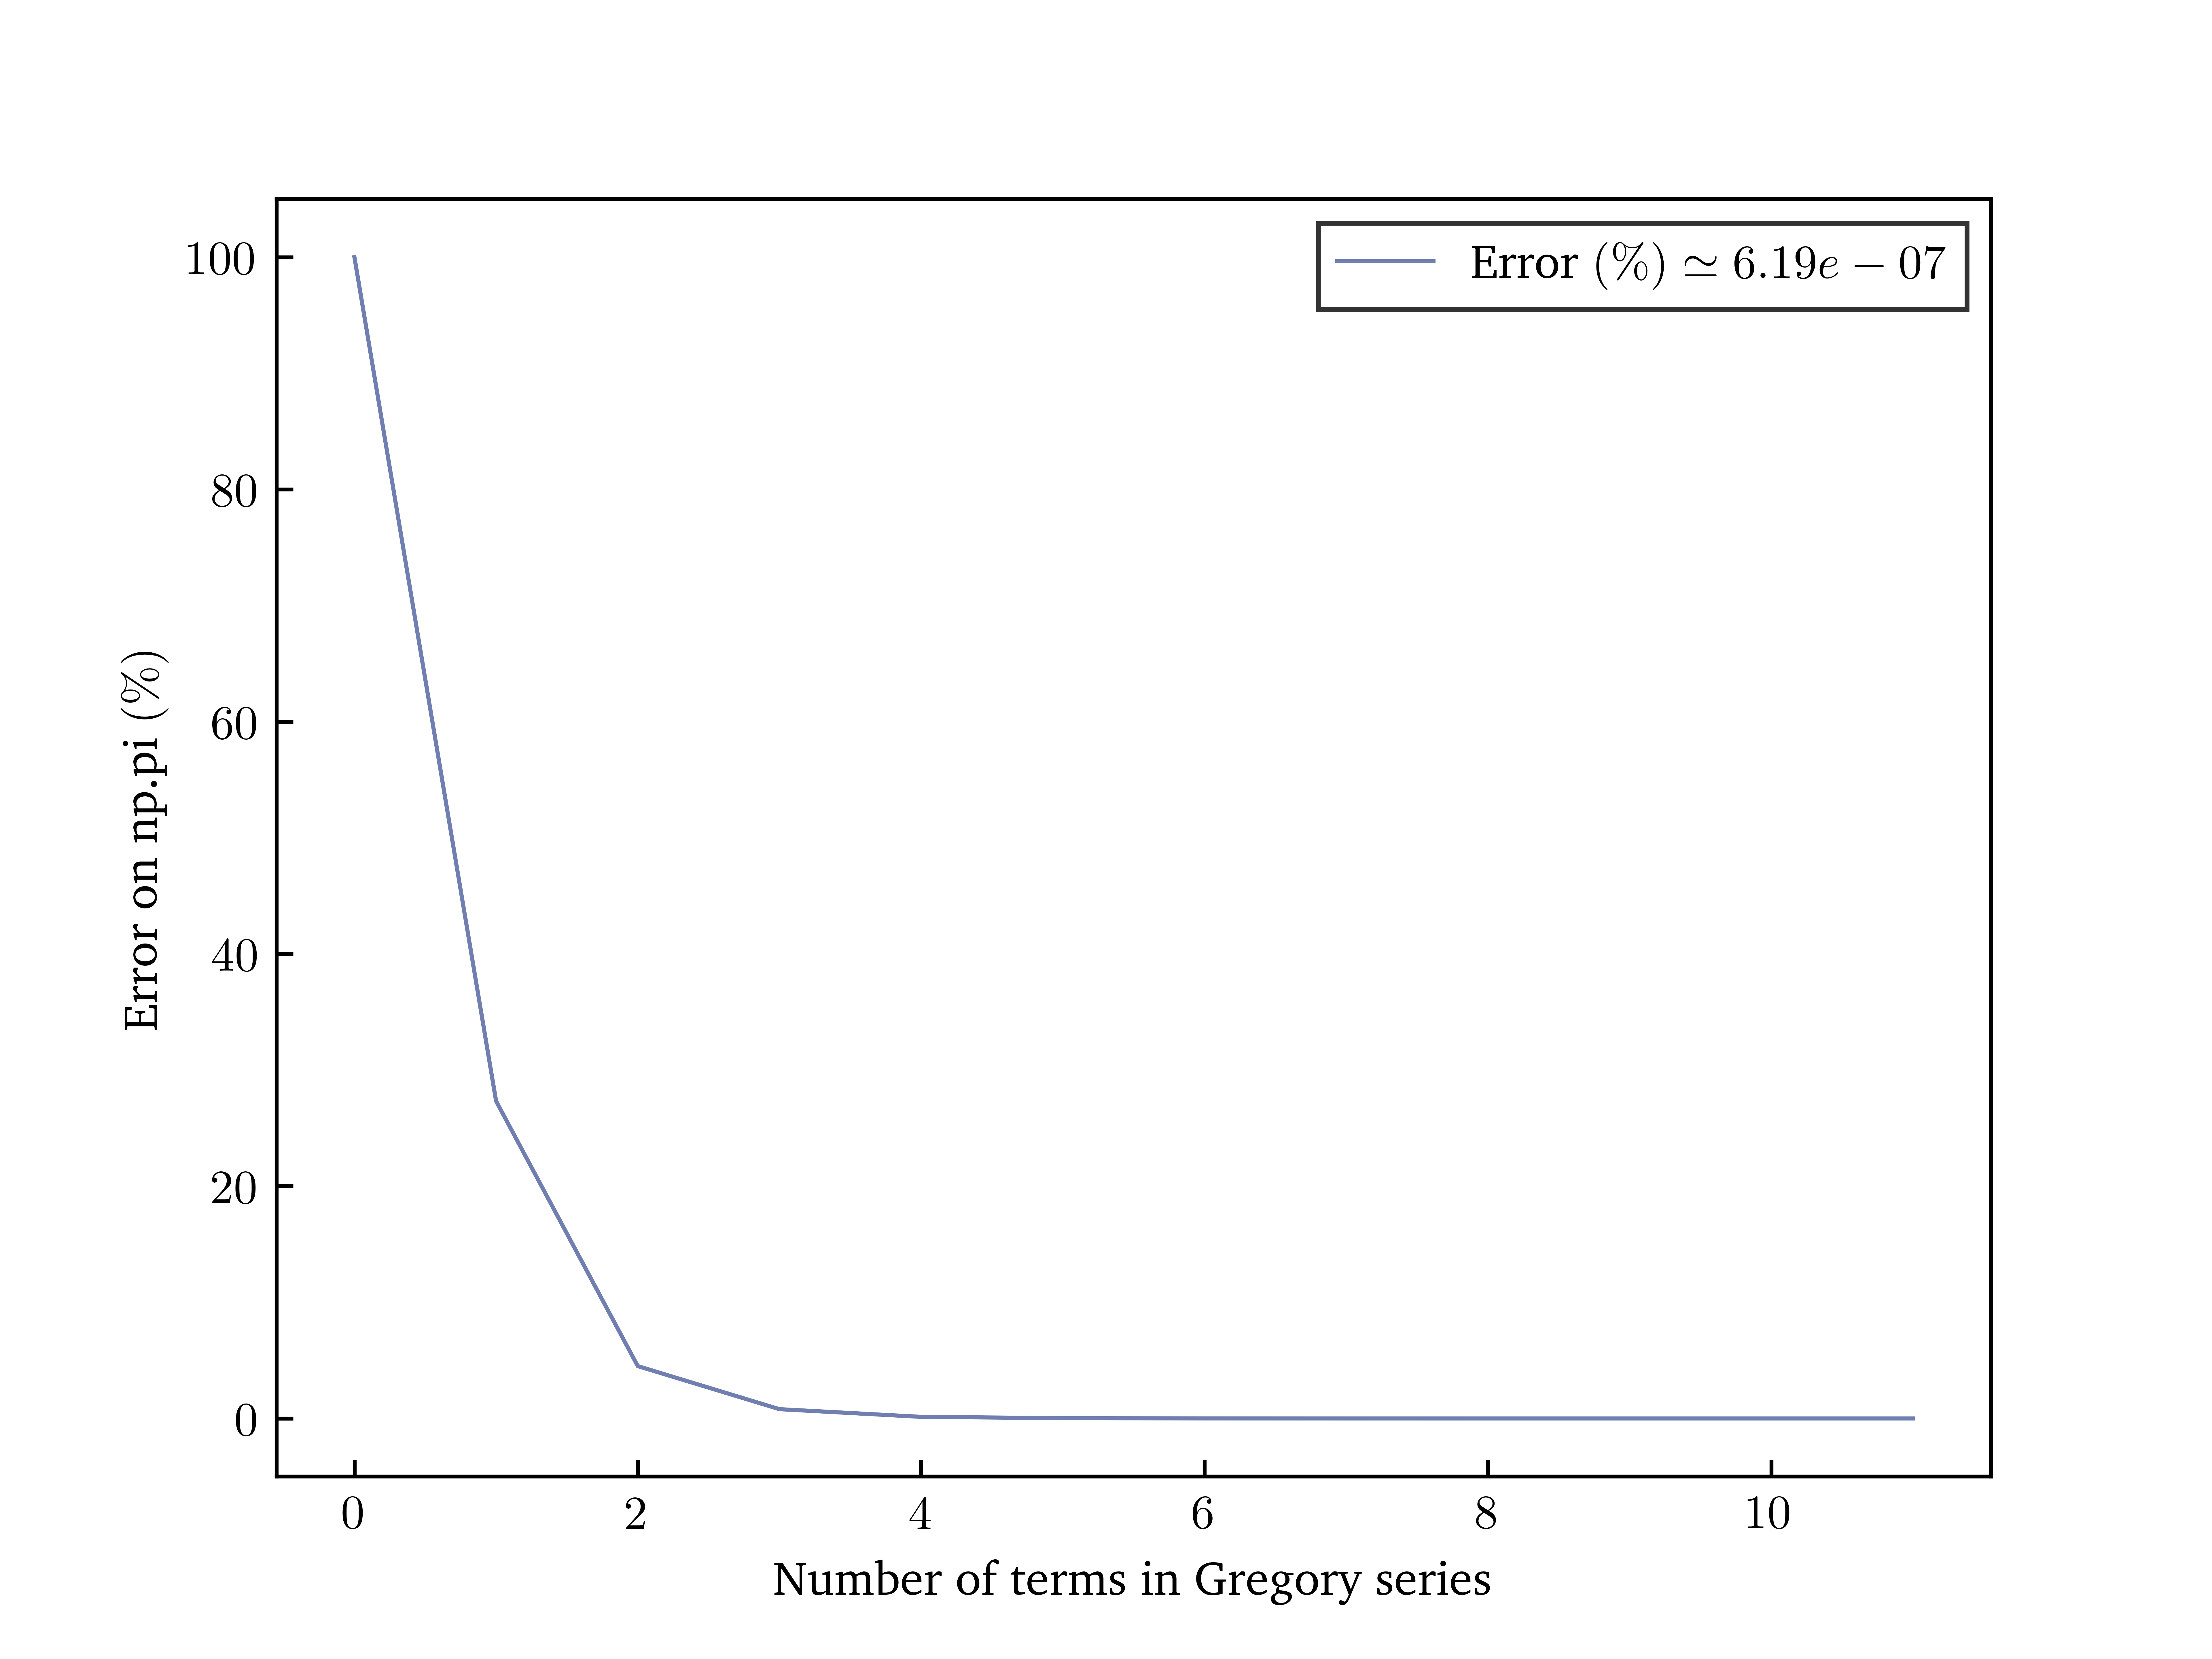
\includegraphics[scale=0.4]{figs/error_percentage.png}
        \caption{Erreur sur l'extrapolation de la série de Gregory (en prenant
        les 12 premiers termes) via l'algorithme epsilon.}
        \label{fig: epsilon_error}
    \end{figure}
    On voit ici sur la figure \ref{fig: epsilon_error} que l'algorithme fait
    effectivement converger la série vers la valeur attendue. On remarque
    qu'avec seulement 5 termes dans la série de Gregory, on peut avoir de très
    bonnes estimations
    \begin{align*}
        \frac{\text{estimation}}{\text{np.pi}}\cdot 100 \simeq
        \frac{3.142342342342342}{3.141592653589793}\cdot 100 \simeq  0.024\%
    \end{align*}


    \section{Théorème d'unicité} \label{sec: annexe_uniqueness}
    \begin{figure}[h!]
        \centering
        \includegraphics[scale=0.4]{figs/trajectories/unicity_lorenz.png}
        \caption{Démonstration qualitative du théorème d'unicité des solutions
        d'équations différentielles ordinaires du premier ordre à l'aide d'une
    trajectoire de l'attracteur de Lorenz.}
        \label{fig: lorenz_uniqueness}
    \end{figure}


    \bibliography{refs}

\end{document}
